\documentclass[a5paper,20pt]{book}
% Det er her vi sætter margener. Pakken geometry giver også adgang til andet.
\usepackage[a5paper, inner=10mm, outer=10mm, top=10mm, bottom=10mm]{geometry}
% Nødvendigt for at få chemfig til at virke.
\usepackage{tikz}
% Sætter de kemiske formler
\usepackage{chemformula}
% Sikrer at vi kan bruge danske specialtegn
\usepackage[utf8]{inputenc}
% Sætter strukturerne
\usepackage{mol2chemfig}
\usepackage{chemfig}
% Font-encoding, bl.a. det tyske dobbelt-s
\usepackage[T1]{fontenc}
% for at kunne inkludere pdf'ere
\usepackage{pdfpages}
% For at kunne styre sidelayhout og den slags.
\usepackage{titlesec}

% Adgang til tabeller der strækker sig over mere end en side.
\usepackage{longtable}




% Hvor vi selv styrer ting
\usepackage{dshk}


\begin{document}

\pagenumbering{gobble}

\begin{center}
\begin{bf}
\Huge{Kemiske småforsøg}
\end{bf}

\hfill

\hfill

Tilrettelagt og redigeret af

\textit{Asbjørn Petersen \& Christian B. Knudsen}

\vspace*{\fill}
Udgivet af

Dansk Selskab for Historisk Kemi

2019
\end{center}

\pagenumbering{roman}
Kemiske småforsøg
Copyright (c) 2019, Dansk Selskab for Historisk Kemi.
Tryk: Et eller andet sted
Trykt i Danmark 2019
ISBN: tretten cifre

Forside illustration



Dansk Selskab for historisk Kemi
Bestyrelseslisten

\chapter{Forord.}

Bostrups klumme. Interessante forsøg. 100 året for Dansk Kemi. Dansk selskab for historisk kemi.
 Og sådan noget.

\pagenumbering{arabic}
\tableofcontents

\pdf{pdfs/1979-60-1-34.pdf}

\emne{Forsøg der belyser opløselighedsproduktet}
\danskkemi{}
\forfatter{Niels Berg}

1. Blyjodid, \ch{PbI2}, er velegnet til at demonstrere virkningen af fælles ioner
på opløseligheden.
Fremstilling af blyjodid: Opløs 1,0 g Pb(NO3)2 i 300 ml kogende vand og tilsæt
en opløsning af 4,0 g kaliumjodid i lidt vand. Udfældes der herved blyjodid,
varmes indtil alt er gået i opløsning. Af den farveløse opløsning udskilles
det gule blyjodid ved afkøling.
Blyjodid suges fra på glasfilter og vaskes et par gange med vand. Noget af
det endnu våde PbI2 kommes i en medicinflaske (500 ml), og efter tilsætning af
vand lukkes flasken med prop og rystes i 10 min.

I hvert af 2 cylinderglas kommes 50 ml af den (filtrerede) mættede opløsning
af PbI2.
Til det ene cylinderglas sættes lidt KI-opløsning. Der udfældes straks PbI2.
Til det andet cylinderglas sættes 1 ml mættet blynitrat-opløsning. Der Udfældes
langsomt større krystaller af PbI2.

Anm: 50 ml \ch{PbI2} + 1/2 ml \ch{Pb(NO3)}, giver fældning.
50 ml \ch{PbI2} + 1 ml \ch{Pb(NO3)}, giver fældning
50 ml \ch{PbI2} + 2 ml \ch{Pb(NO3)}, giver fældning
50 ml \ch{PbI2} + 4 ml \ch{Pb(NO3)}, giver ikke fældning

2. Sølvacetat, \ch{CH3COOAg}, kan bruges til et analogt forsøg:
0,50 g sølvnitrat og 0,40 g krystallinsk natriumacetat, CH3COONa,3H2O *) opløses
hver for sig i 25 ml vand, hvorpå opløsningerne blandes. Der fås en omtrent
mættet opløsning af sølvacetat. At denne desuden indeholder Na+ og NO3- spiller
ingen rolle. Nogle få ml tages fra for at kontrollere at der ikke sker
udfældning i blandingen.
Resten deles i 2 lige store dele. Den ene fældes med 2,0 g AgNO3, den anden med
1,6 g CH3COONa3H2O **), begge salte opløst i 5 ml vand. Der udfældes CH3COOAg
i begge portioner.

*) eller 0,24 g vandfast salt, **) eller 0,97 g vandfrit salt

\pdf{pdfs/1979-60-1-34.pdf}

\emne{}
\danskkemi{}
\forfatter{}

\deloverskrift{}

\pdf{pdfs/1979-60-2-58.pdf}

\emne{}
\danskkemi{}
\forfatter{}

\deloverskrift{}

\pdf{pdfs/1979-60-2-58.pdf}

\emne{}
\danskkemi{}
\forfatter{}

\deloverskrift{}

\pdf{pdfs/1979-60-2-58.pdf}

\emne{}
\danskkemi{}
\forfatter{}

\deloverskrift{}

\pdf{pdfs/1979-60-2-58.pdf}

\emne{}
\danskkemi{}
\forfatter{}

\deloverskrift{}

\pdf{pdfs/1979-60-3-94.pdf}

\emne{}
\danskkemi{}
\forfatter{}

\deloverskrift{}

\pdf{pdfs/1979-60-3-94.pdf}

\emne{}
\danskkemi{}
\forfatter{}

\deloverskrift{}

\pdf{pdfs/1979-60-3-94.pdf}

\emne{}
\danskkemi{}
\forfatter{}

\deloverskrift{}

\pdf{pdfs/1979-60-4-118.pdf}

\emne{}
\danskkemi{}
\forfatter{}

\deloverskrift{}

\pdf{pdfs/1979-60-5-154.pdf}

\emne{}
\danskkemi{}
\forfatter{}

\deloverskrift{}

\pdf{pdfs/1979-60-5-154.pdf}

\emne{}
\danskkemi{}
\forfatter{}

\deloverskrift{}

\pdf{pdfs/1979-60-67-186.pdf}

\emne{}
\danskkemi{}
\forfatter{}

\deloverskrift{}

\pdf{pdfs/1979-60-67-186.pdf}

\emne{}
\danskkemi{}
\forfatter{}

\deloverskrift{}

\pdf{pdfs/1979-60-8-214.pdf}

\emne{}
\danskkemi{}
\forfatter{}

\deloverskrift{}

\pdf{pdfs/1979-60-8-214.pdf}

\emne{}
\danskkemi{}
\forfatter{}

\deloverskrift{}

\pdf{pdfs/1979-60-9-254.pdf}

\emne{}
\danskkemi{}
\forfatter{}

\deloverskrift{}

\pdf{pdfs/1979-60-9-254.pdf}

\emne{}
\danskkemi{}
\forfatter{}

\deloverskrift{}

\pdf{pdfs/1979-60-10-286.pdf}

\emne{}
\danskkemi{}
\forfatter{}

\deloverskrift{}

\pdf{pdfs/1979-60-10-286.pdf}

\emne{}
\danskkemi{}
\forfatter{}

\deloverskrift{}

\pdf{pdfs/1979-60-11-322.pdf}

\emne{}
\danskkemi{}
\forfatter{}

\deloverskrift{}

\pdf{pdfs/1979-60-11-322.pdf}

\emne{}
\danskkemi{}
\forfatter{}

\deloverskrift{}

\pdf{pdfs/1979-60-11-322.pdf}

\emne{}
\danskkemi{}
\forfatter{}

\deloverskrift{}

\pdf{pdfs/1979-60-11-322.pdf}

\emne{}
\danskkemi{}
\forfatter{}

\deloverskrift{}

\pdf{pdfs/1979-60-12-354.pdf}

\emne{}
\danskkemi{}
\forfatter{}

\deloverskrift{}

\pdf{pdfs/1979-60-12-354.pdf}

\emne{}
\danskkemi{}
\forfatter{}

\deloverskrift{}

\pdf{pdfs/1979-60-12-354.pdf}

\emne{}
\danskkemi{}
\forfatter{}

\deloverskrift{}

\pdf{pdfs/1979-60-12-354.pdf}

\emne{}
\danskkemi{}
\forfatter{}

\deloverskrift{}

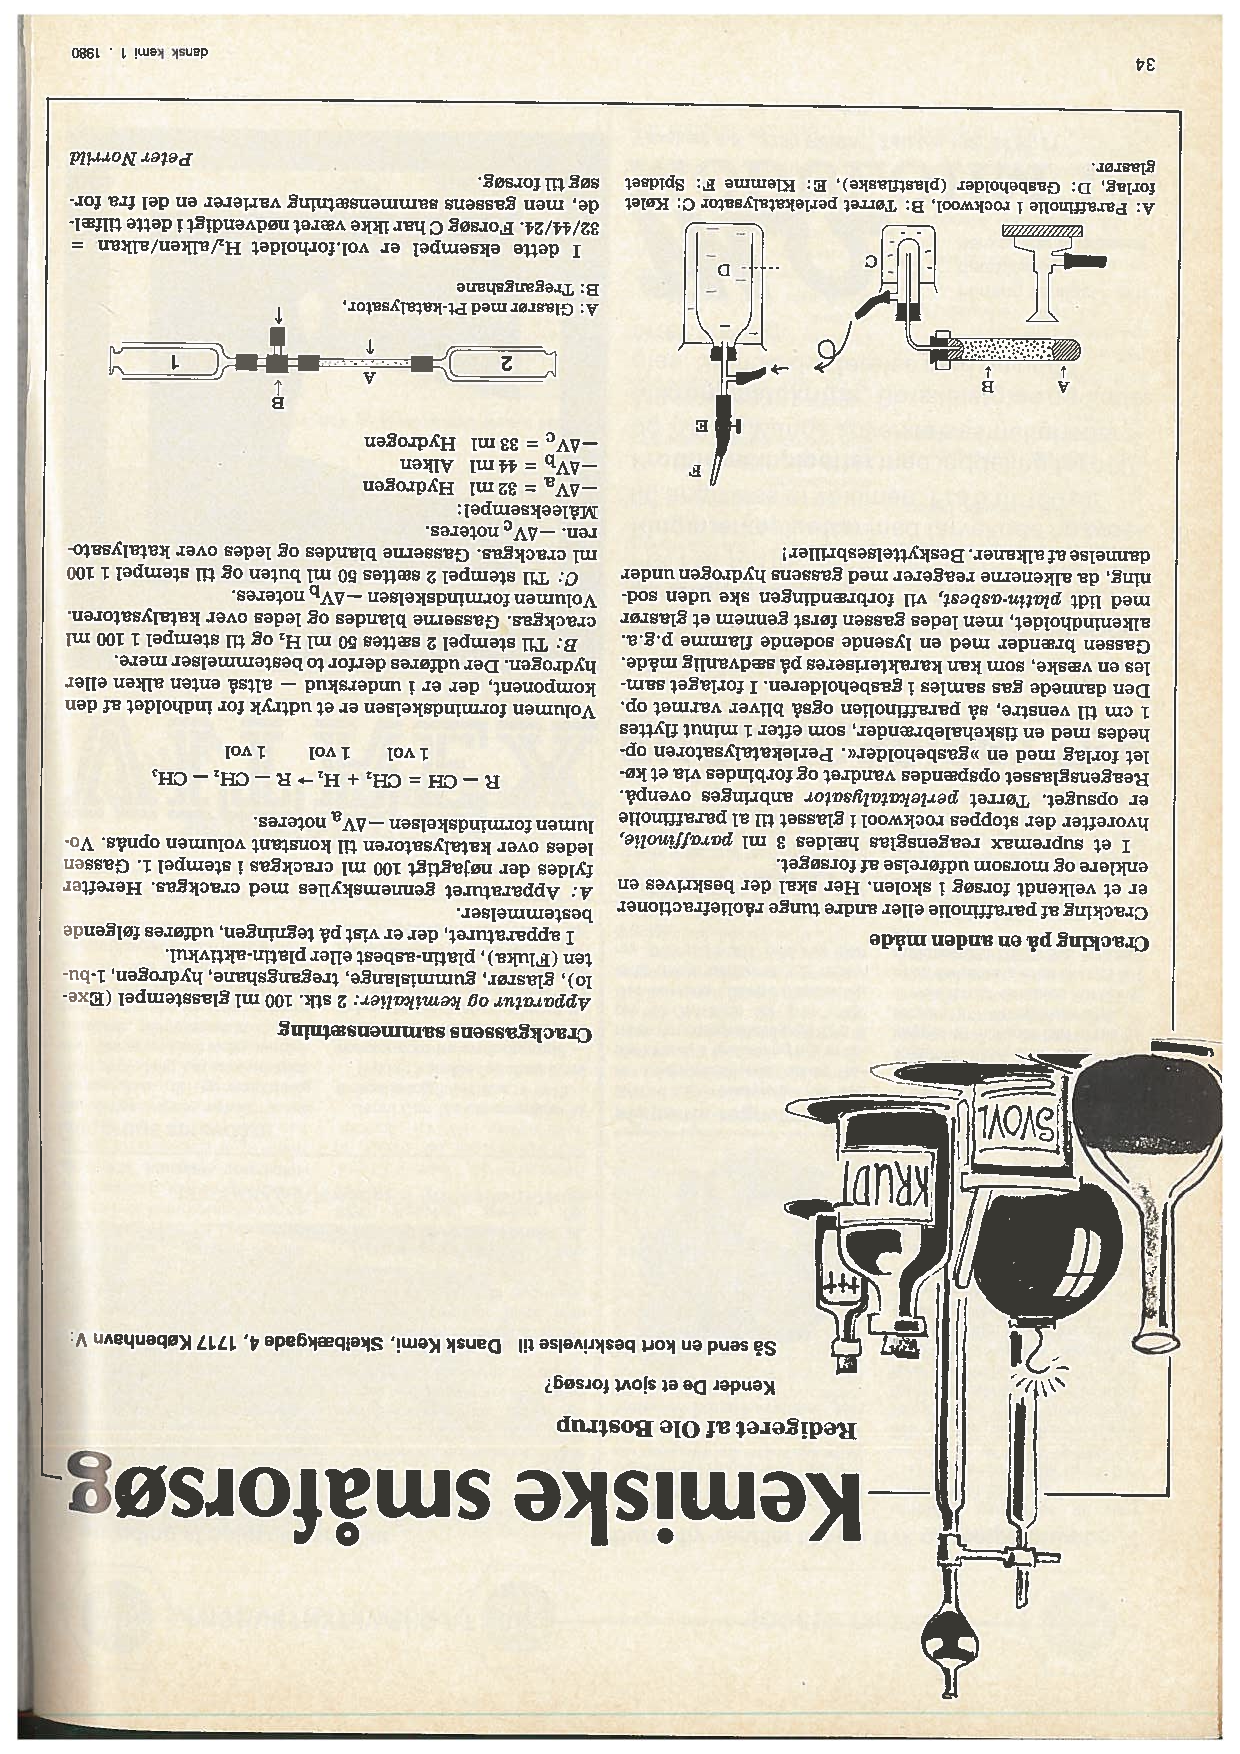
\includepdf[pages=-]{pdfs/1980-61-1-34.pdf}
\emne{Cracking på en anden måde}
\danskkemi{ dansk kemi vol 61 iss 1 p 34}
\forfatter{Peter Norrild}



Cracking af paraffinolie eller andre tunge råoliefractioner er et velkendt
forsøg i skolen. Her skal der beskrives en enklere og morsom udførelse af
forsøget.

I et supremax reagensglas hældes 3 ml paraffinolie, hvorefter der stoppes
rockwool i glasset til al paraffinolie er opsuget. Tørret perlekatalysator
anbringes ovenpå. reagensglasset opspændes vandret og forbindes via et kølet
forlag med en "gasbeholder". perlekatalysatoren ophedes med en fiskehalebrænder,
som efter 1 minut flyttes 1 cm til venstre, så paraffinolien også bliver varmet
op. Den dannede gas samles i gasbeholderen. I forlaget samles en væske, som kan
karakteriseres på sædvanlig måde. Gassen brænder med en lysende sodende flamme
p.g.a. alkenindholdet, men ledes gassen først gennem et glasrør med lidt
platin-asbest, vil forbrændingen ske uden sodning, da alkenerne reagerer med
gassens hydrogen under dannelse af alkaner. Beskyttelsesbriller!

\deloverskrift{Crackgassens sammensætning}

Apparatur og kemikalier: 2 stk. 100 ml glasstempel (Exelo), glasrør,
gummislange, tregangshane, hydrogen, 1-buten (Fluka), platin-asbest
eller platin-aktivkul.
I apparaturet, der er vist på tegningen, udføres følgende bestemmelser.
A: Apparaturet gennemskylles med crackgas. Herefter fyldes der nøjagtigt
100 ml crackgas i stempel 1. Gassen ledes over katalysatoren til konstant
volumen opnås. Volumen formindskelsen -Delta Va noteres.

R-CH=CH2 + H2 -> R-CH2-CH3
1 vol 1 vol 1 vol

Volumen formindskelsen er et udtryk for indholdet af den komponent, der
er i underskud - altså enten alekn eller hydrogen. Der udføres derfor to bestemmelser mere.
B: Til stempel 2 sættes 50 ml H2 og til stempel 1 100 ml crackgas.
Gassernes blandes og ledes over katalysatoren. Volumen formindskelsen
-Delta Vb noteres.
C: Til stempel 2 sættes 50 ml buten og til stempel 1 100 ml
crackgas. Gasserne blandes og ledes over katalysatoren. - Delta Vc
noteres.
Måleeksempel:
- Delta Va = 32 ml Hydrogen
-Delta Vb = 44 ml Alken
-Delta Vc = 33 ml Hydrogen

I dette eksempel er vol.forholdet H2/alken/alkan = 32/44/24.
Forsøg C har ikke været nødvendigt i dette tilfælde, men gassens
sammensætning varierer en del fra forsøg til forsøg.

noter til illustration 1:
A: Paraffinolie i rockwool, B: Tørret perlekatalysator D: Kølet forlag,
D: Gasbeholder (plastflaske), E: Klemme F: Spidset glasrør.

Noter til illustration 2:
A: Glasrør med Pt-katalysator,
B: tregangshane

 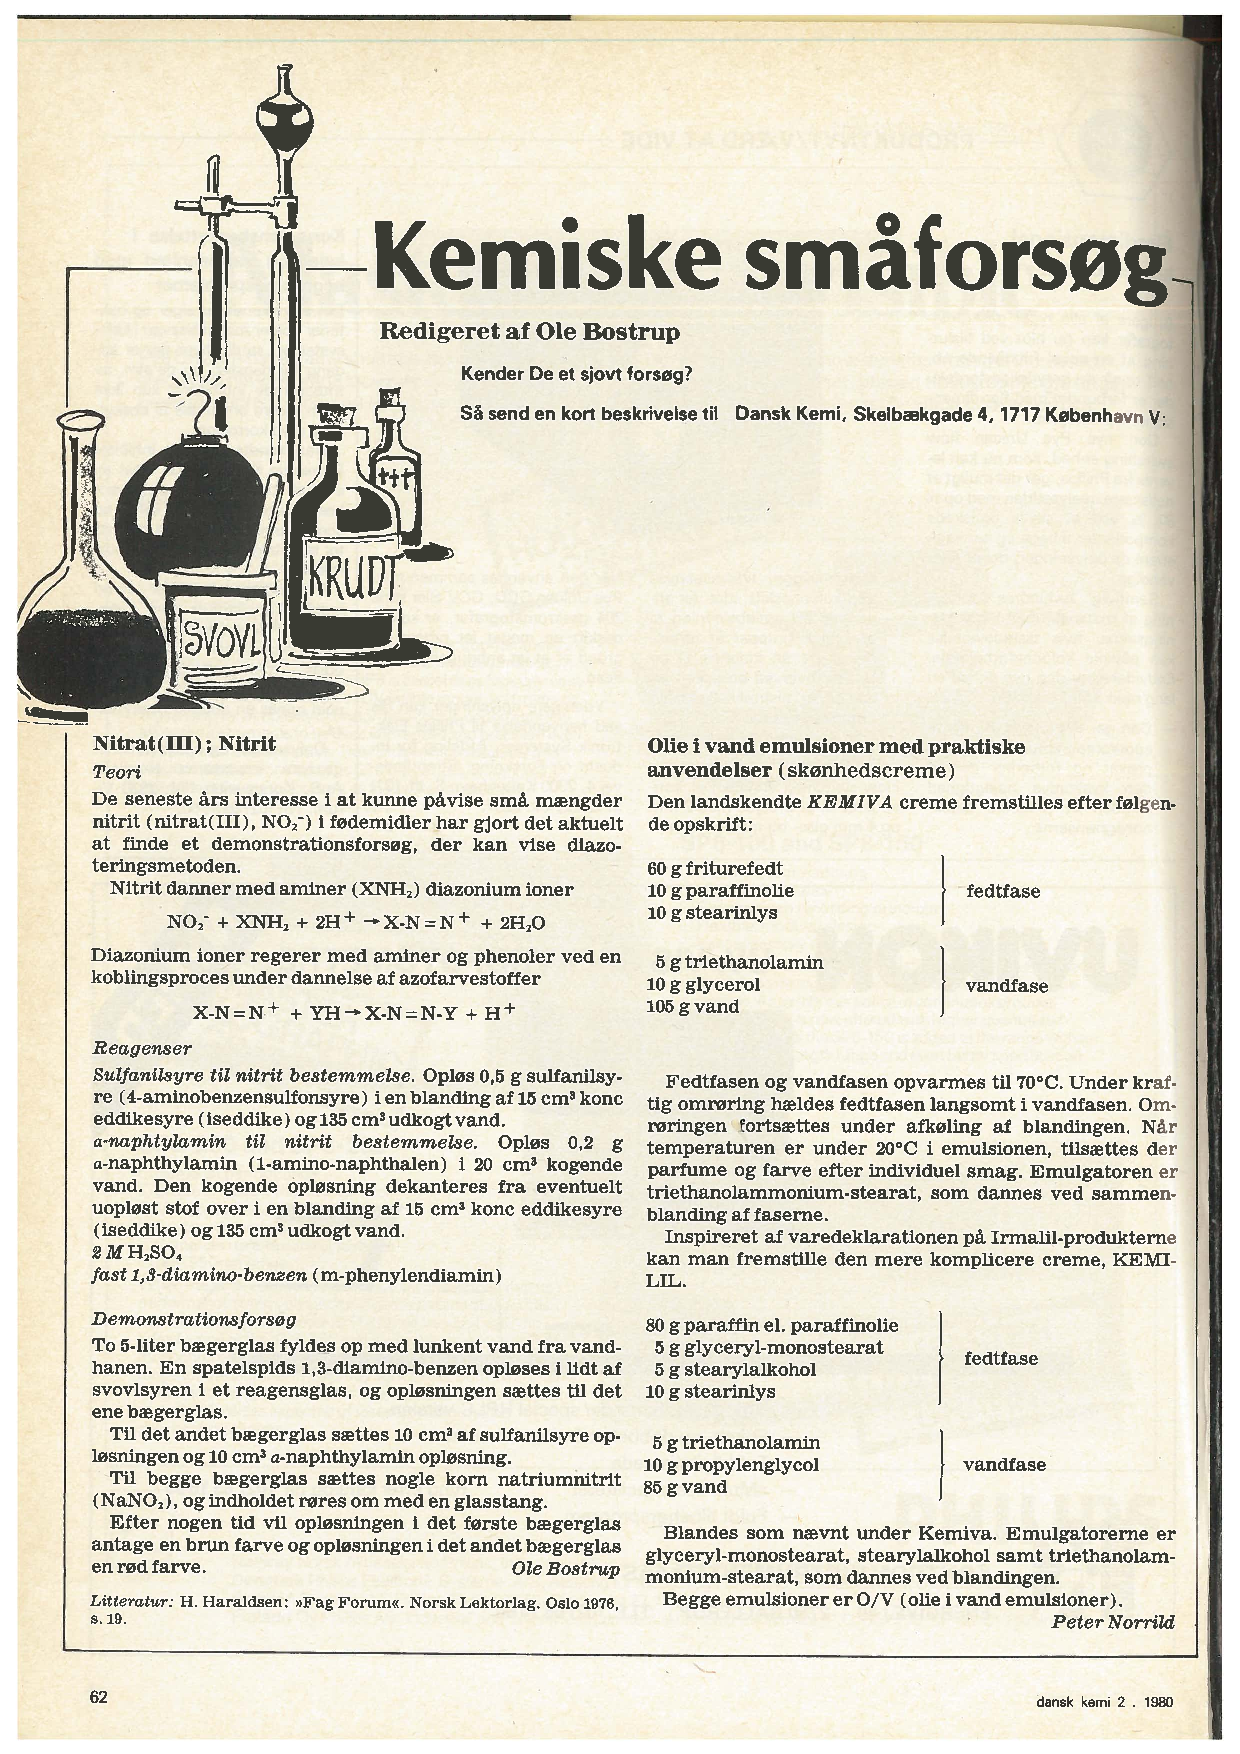
\includepdf[pages=-]{pdfs/1980-61-2-62.pdf}

\emne{Nitrat (III); Nitrit}
dansk kemi vol 61 iss 2 p 62

Teori

De seneste års interesse i at kunne påvise små mængder nitrit (nitrat(III), NO2-) i fødemidler har gjort det aktuelt at finde et
demonstationsforsøg, der kan vise diazoteringsmetoden.
Nitrit danner med aminer (XNH2) diazonium ioner

\ch{NO2- + X NH2 + 2 H+ -> X-N=N+ + 2 H2O}

Diazonium ioner regerer med aminer og phenoler ved en koblingsproces
under dannelse af azofarvestoffer
\ch{X-N=N+ + YH -> X-N=N-Y + H+}

Reagenser
Sulfanilsyre til nitrit bestemmelse. Opløs 0,5 g sulfanilsyre
(4-aminobenzensulfonsyre) i en blanding af 15 cm3 konc eddikesyre
(iseddike) og 135 cm3 udkogt vand.
a-naphtylamin til nitrit bestemmelse. Opløs 0,2 g a-naphthylamin
(1-amino-naphthalen) i 20 cm3 kogende vand. Den kogende opløsning
dekanteres fra eventuelt uopløst stof oer i en blanding af 15 cm3
konc eddikesyre (iseddike) og 135 cm3 udkogt vand.
2 M H2SO4
fast 1,3-diamino-benzen (m-phenylendiamin)

Demonstrationsforsøg
To 5-liter bægerglas fyldes op med lunkent vand fra vandhanen.
En spatelspids 1,3-diamino-benzen opløses i lidt af svovlsyre i et
reagensglas, og opløsningen sættes til det ene bægerglas.
Til det andet bægerglas sættes 10 cm3 af sulfanilsyre opløsningen og
10 cm3 a-naphthylamin opløsning.
Til begge bægerglas sættes nogle korn natriumnitrit (NaNO2) og indholdet
røres om med en glasstang.
Efter nogen tid vil opløsningen i det første bægerglas antage en
brun farve og opløsningen i det andet bægerglas en rød farve.

Forfatter: Ole Bostrup.
Litteratur: H. Haraldsen: "Fag Forum". Norsk Lektorlag. Oslo 1976, s. 19.

 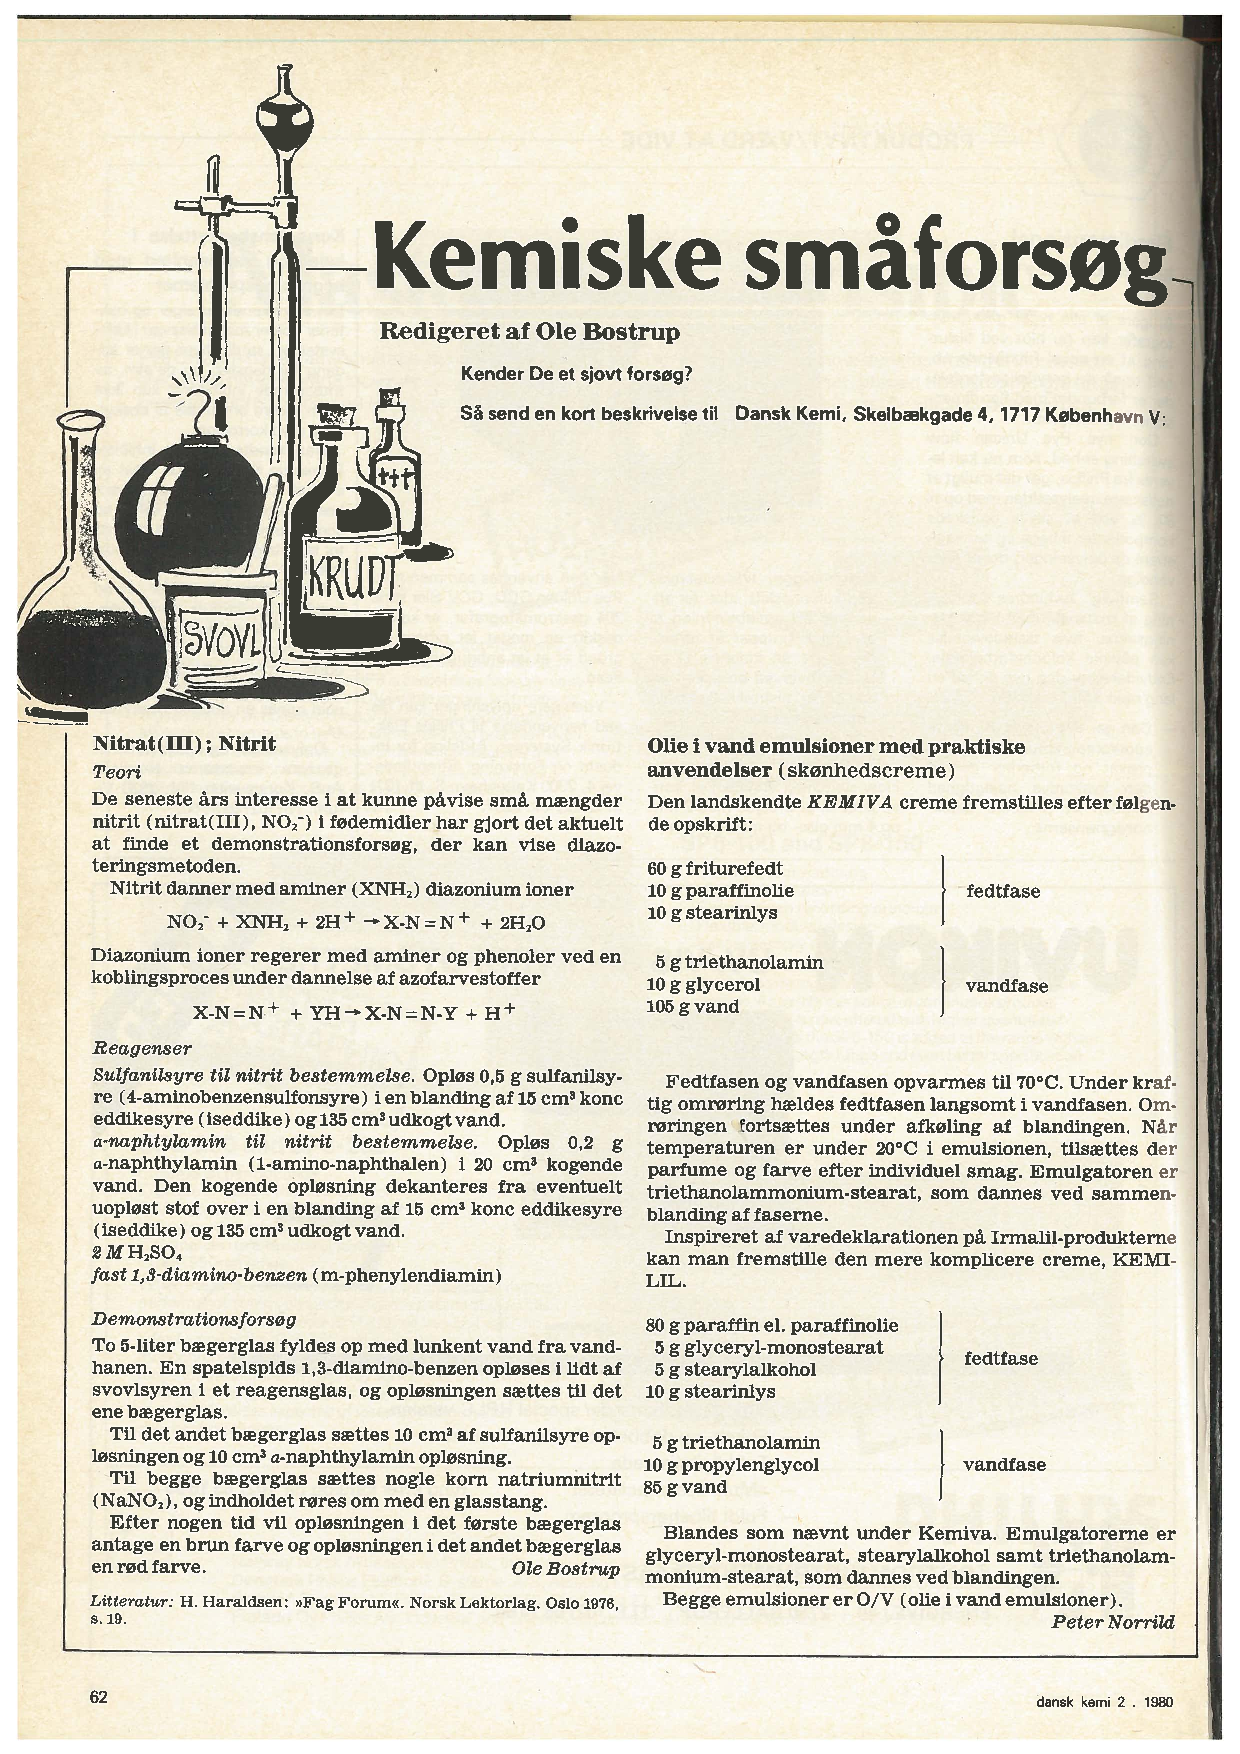
\includepdf[pages=-]{pdfs/1980-61-2-62.pdf}
% dansk kemi vol 61 iss 2 p 62

nr to

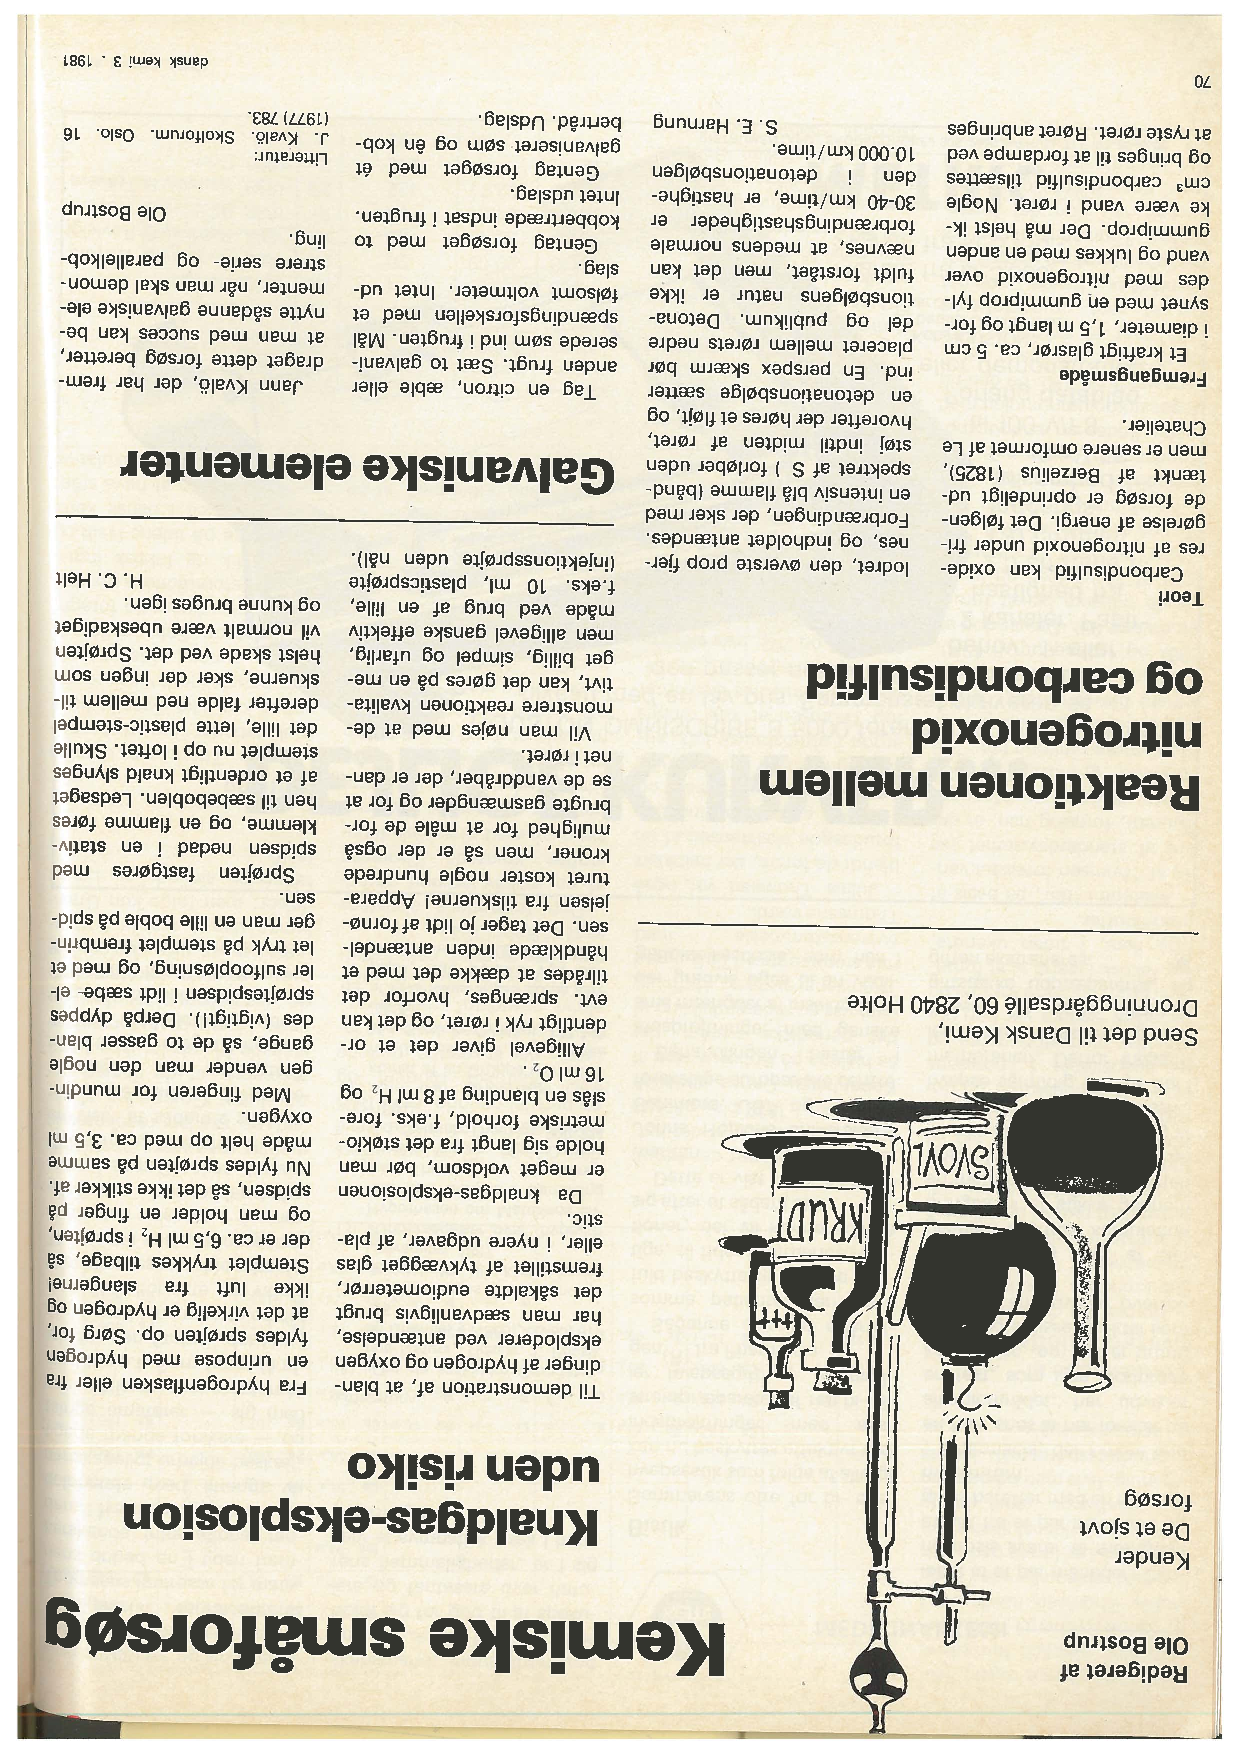
\includepdf[pages=-]{pdfs/1981-62-3-70.pdf}

\emne{Reaktionen mellem nitrogenoxid og carbondisulfid}

\danskkemi{Dansk Kemi 62, 3, 1981, p. 70}

Forfatter: S. E. Harnung

Teori
carbondisulfid kan oxideres af nitrogenoxid under frigørelse af energi. Det
efterfølgende forsøg er oprindeligt udtænkt af Berzelius (1825), men er
senere omformet af Le Chatelier.

Fremgangsmåde

Et kraftigt glasrør, ca. 5 cm i diameter, 1,5 m langt og forsynet med en gummiprop
fyldes med nitrogenoxid over vand og lukkes med en anden gummiprop.
Der må helst ikke være vand i røret. Nogle cm3 carbondisulfid tilsættes og
bringes til at fordampe ved at ryste røret. Røret anbringes lodret, den
øverste prop fjernes, og indholdet antændes. Forbrændingen, der sker med
en intensiv blå flamme (båndspektret af S) forløber uden støj indtil midten af
røret, hvorefter der høres et fløjt, og en detonationsbølge sætter ind.
En perspex skærm bør placeres mellem rørets nedre del og publikum.
detonationsbølgens natur er ikke fuldt forstået, men det kan nævnes, at
medens normale forbrændingshastigheder er 30-40 km/time, er hastigheden i
detonationsbølgen 10.000 km/time.

\include{dele/62-3-c}
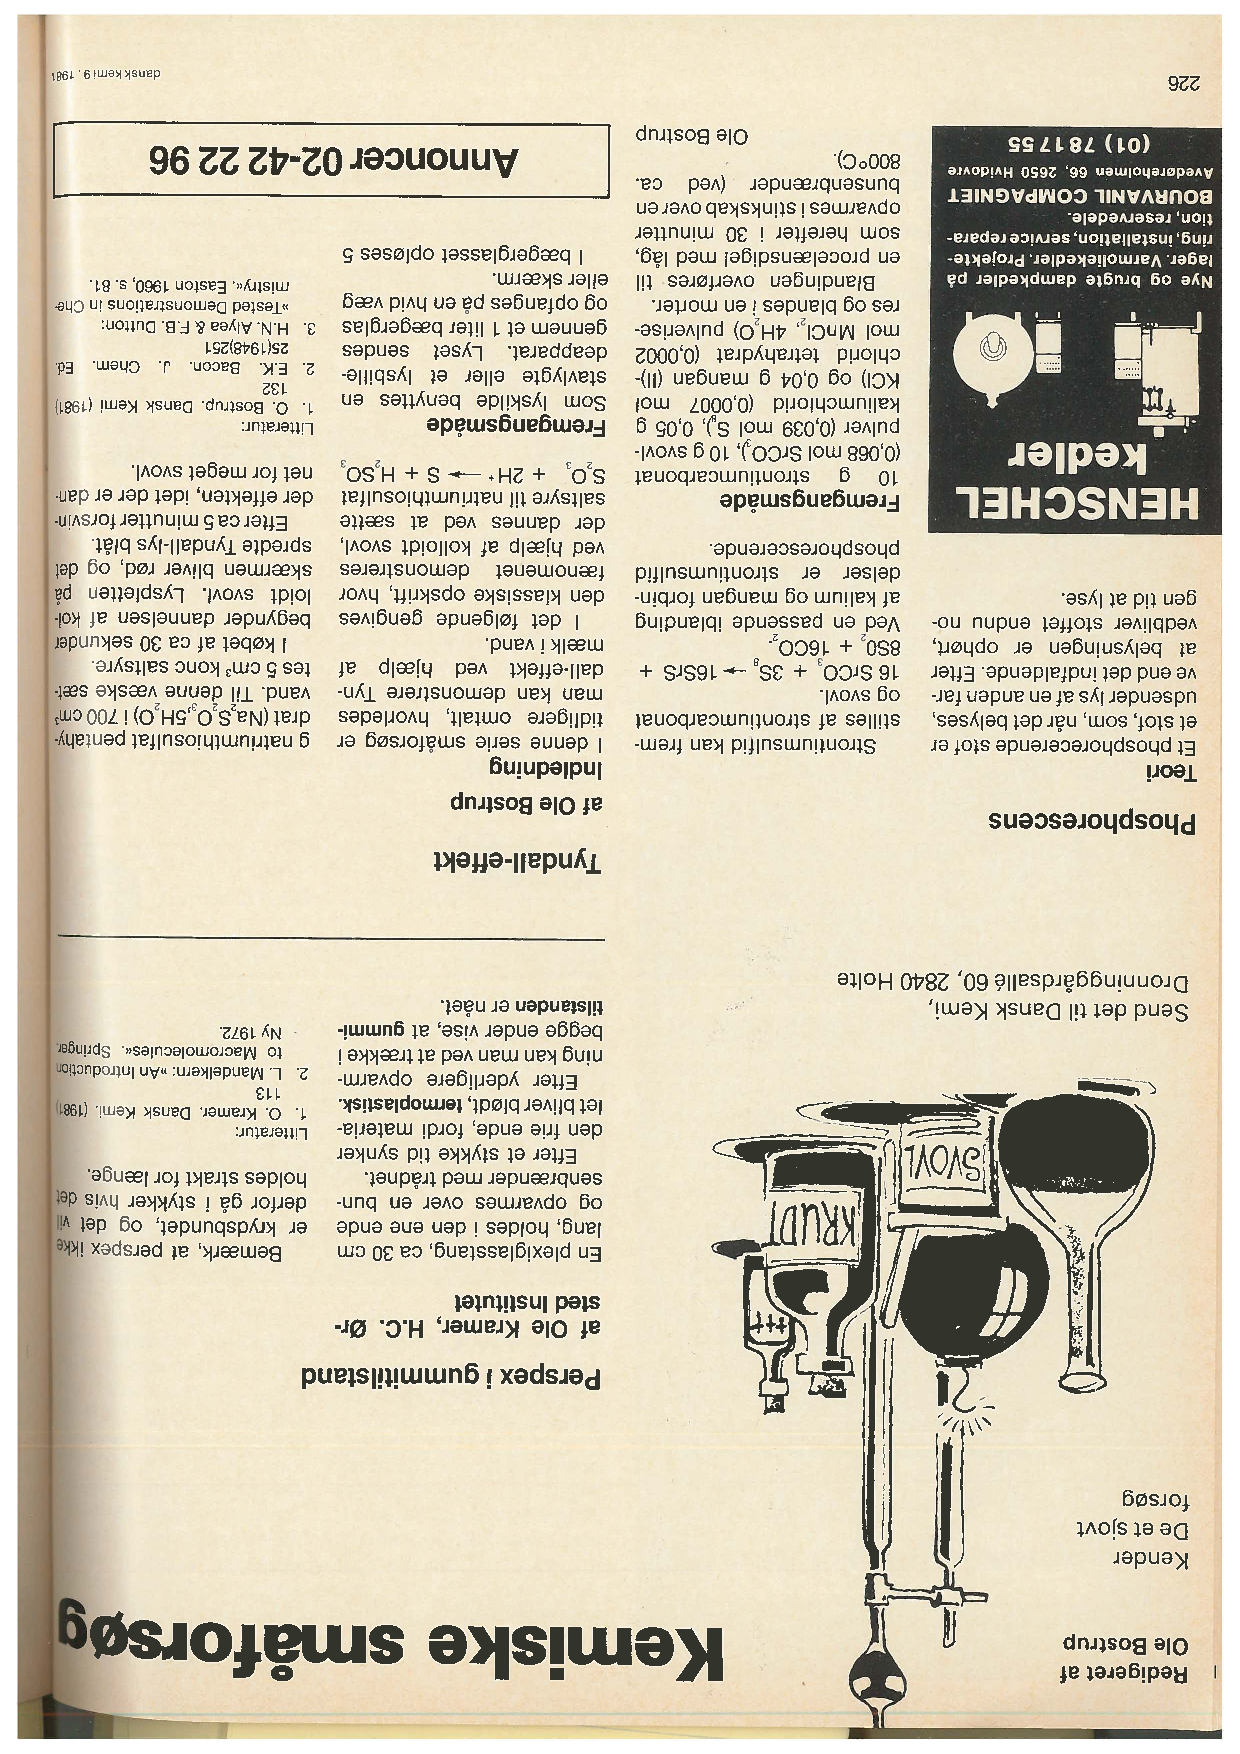
\includepdf[pages=-]{pdfs/1981-62-9-226.pdf}

\emne{Phosphorescens}
\danskkemi{1981-62-9-226}
\forfatter{Ole Bostrup}


\deloverskrift{Teori}

Et phosphorecerende stof er et stof, som, når det
belyses, udsender lys af en anden farve end det
indfaldende. Efter at belysningen er ophørt,
vedbliver stoffet endnu nogen tid at lyse.

Strontiumsulfid kan fremstilles af strontiumcarbonat
og svovl.
\begin{center}
\ch{16 SrCO3 + 2 S8 -> 16 SrS + 8 SO2 + 16 CO2}
\end{center}
Ved en passende iblanding af kalium og mangan
forbindelser er strontiumsulfid phosphorescerende.

\deloverskrift{Fremgangsmåde}

10 g strontiumcarbonat (0,068 mol \ch{SrCO3}), 10 g
svovlpulver (0,039 mol \ch{S8}), 0,05 g kaliumchlorid
(0.0007 mol KCl) og 0,4 g mangan (II)- chlorid
tetrahydrat (0,0002 mol \ch{MnCl2}, \ch{4 H2O}) pulveriseres
og blandes i en morter.
Blandingen overføres til en porcelænsdigel med
låg, som herefter i 30 minutter opvarmes i
stinkskab over en bunsenbrænder (ved ca. 800
gradtegn C).

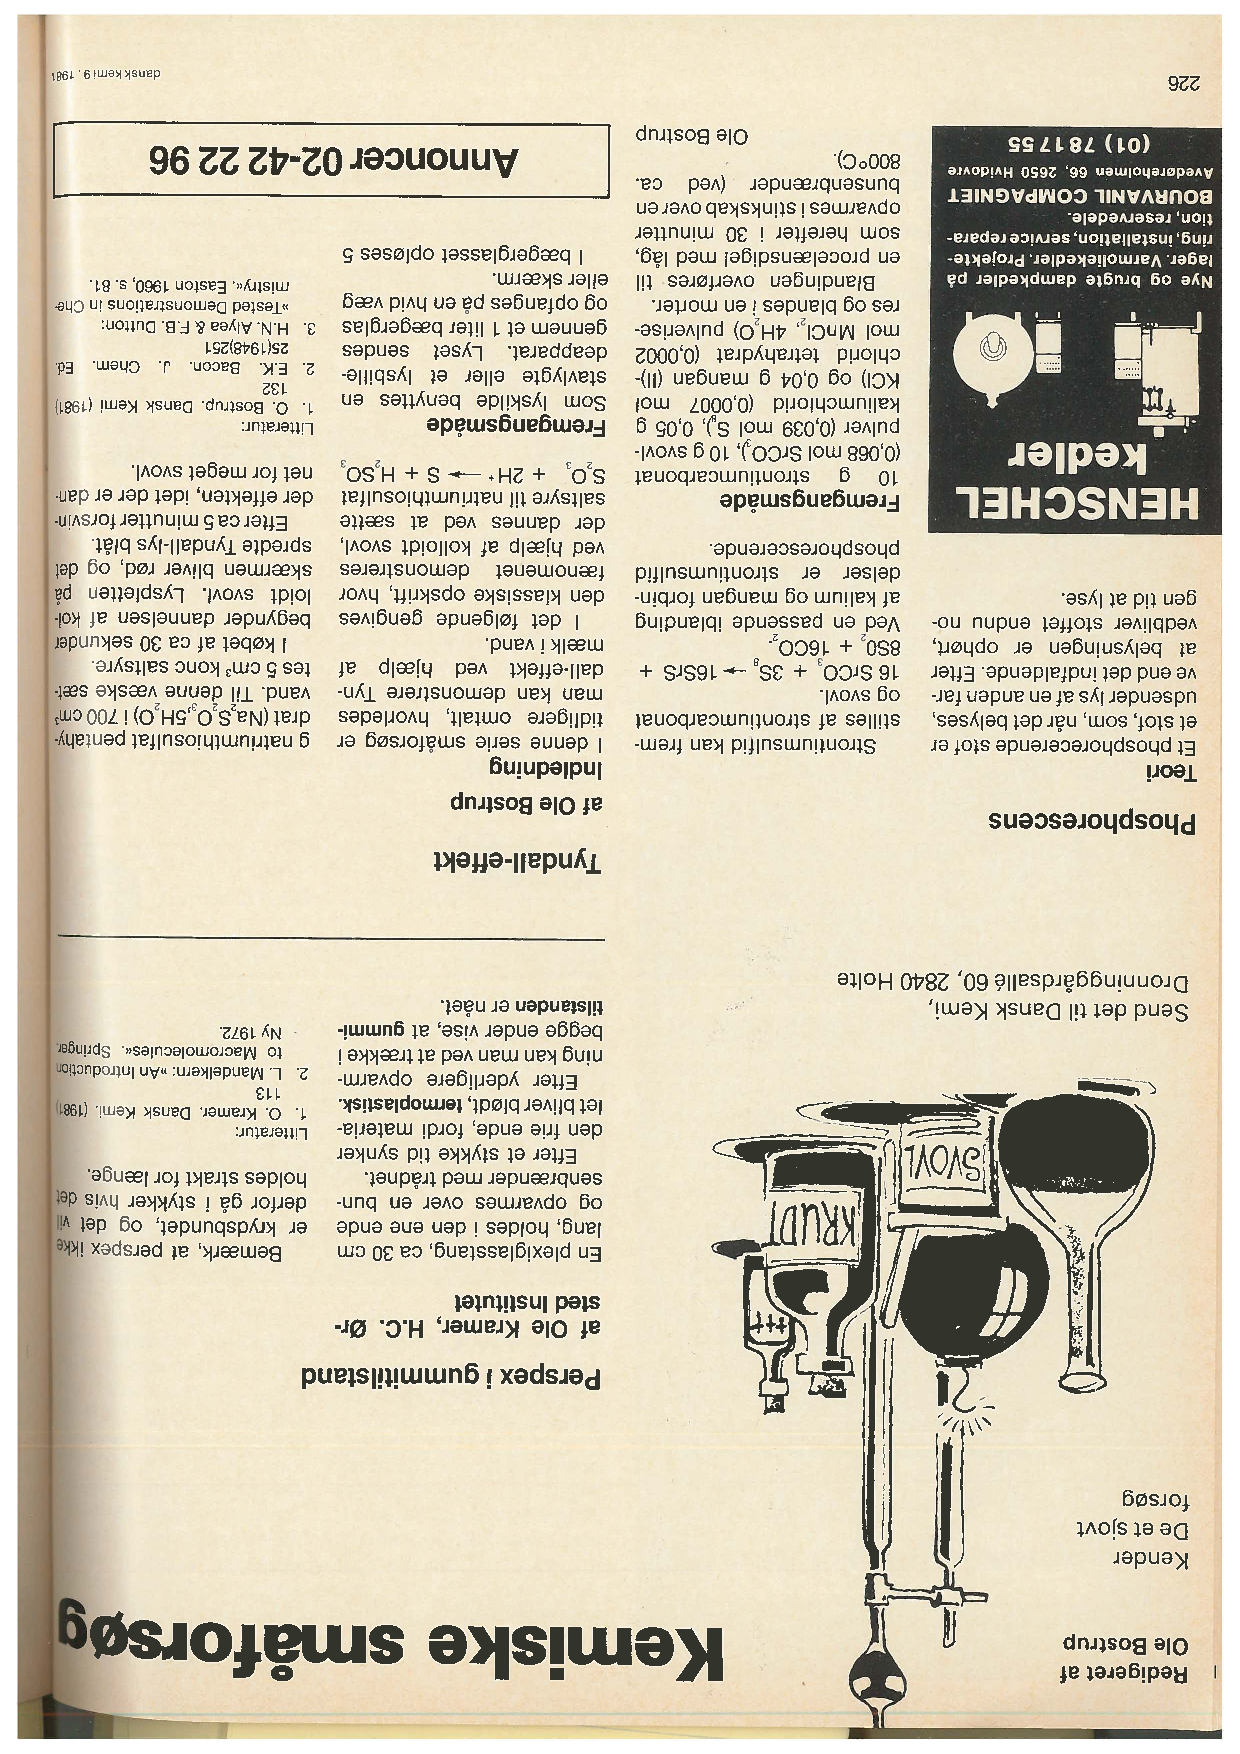
\includepdf[pages=-]{pdfs/1981-62-9-226.pdf}


\emne{Perspex i gummitilstand}
\danskkemi{Dansk Kemi 62, 3, 1981, p. 70}
\forfatter{Ole Kramer, H.C. Ørsted Institutet}

En plexiglasstang, ca 30 cm lang, holdes i den ene ende
og opvarmes over en bunsenbrænder med trådnet.
Efter et stykke tid synker den frie ende, fordi
materialet bliver blødt, \bf{termoplastiks}
Efter yderligere opvarmning kan man ved at trække i begge
ender vise, at \bf{gummitilstanden} er nået.

Bemærk at perspex ikke er krydsbundet, og det vil derfor
gå i stykker hvis det holdes strakt for længe.

Litteratur:
1. O. Kramer. Dansk Kemi, (1981) 113
2. L. Mandelkern: "An Introduction to Macromolecules".
Springer, Ny 1972.

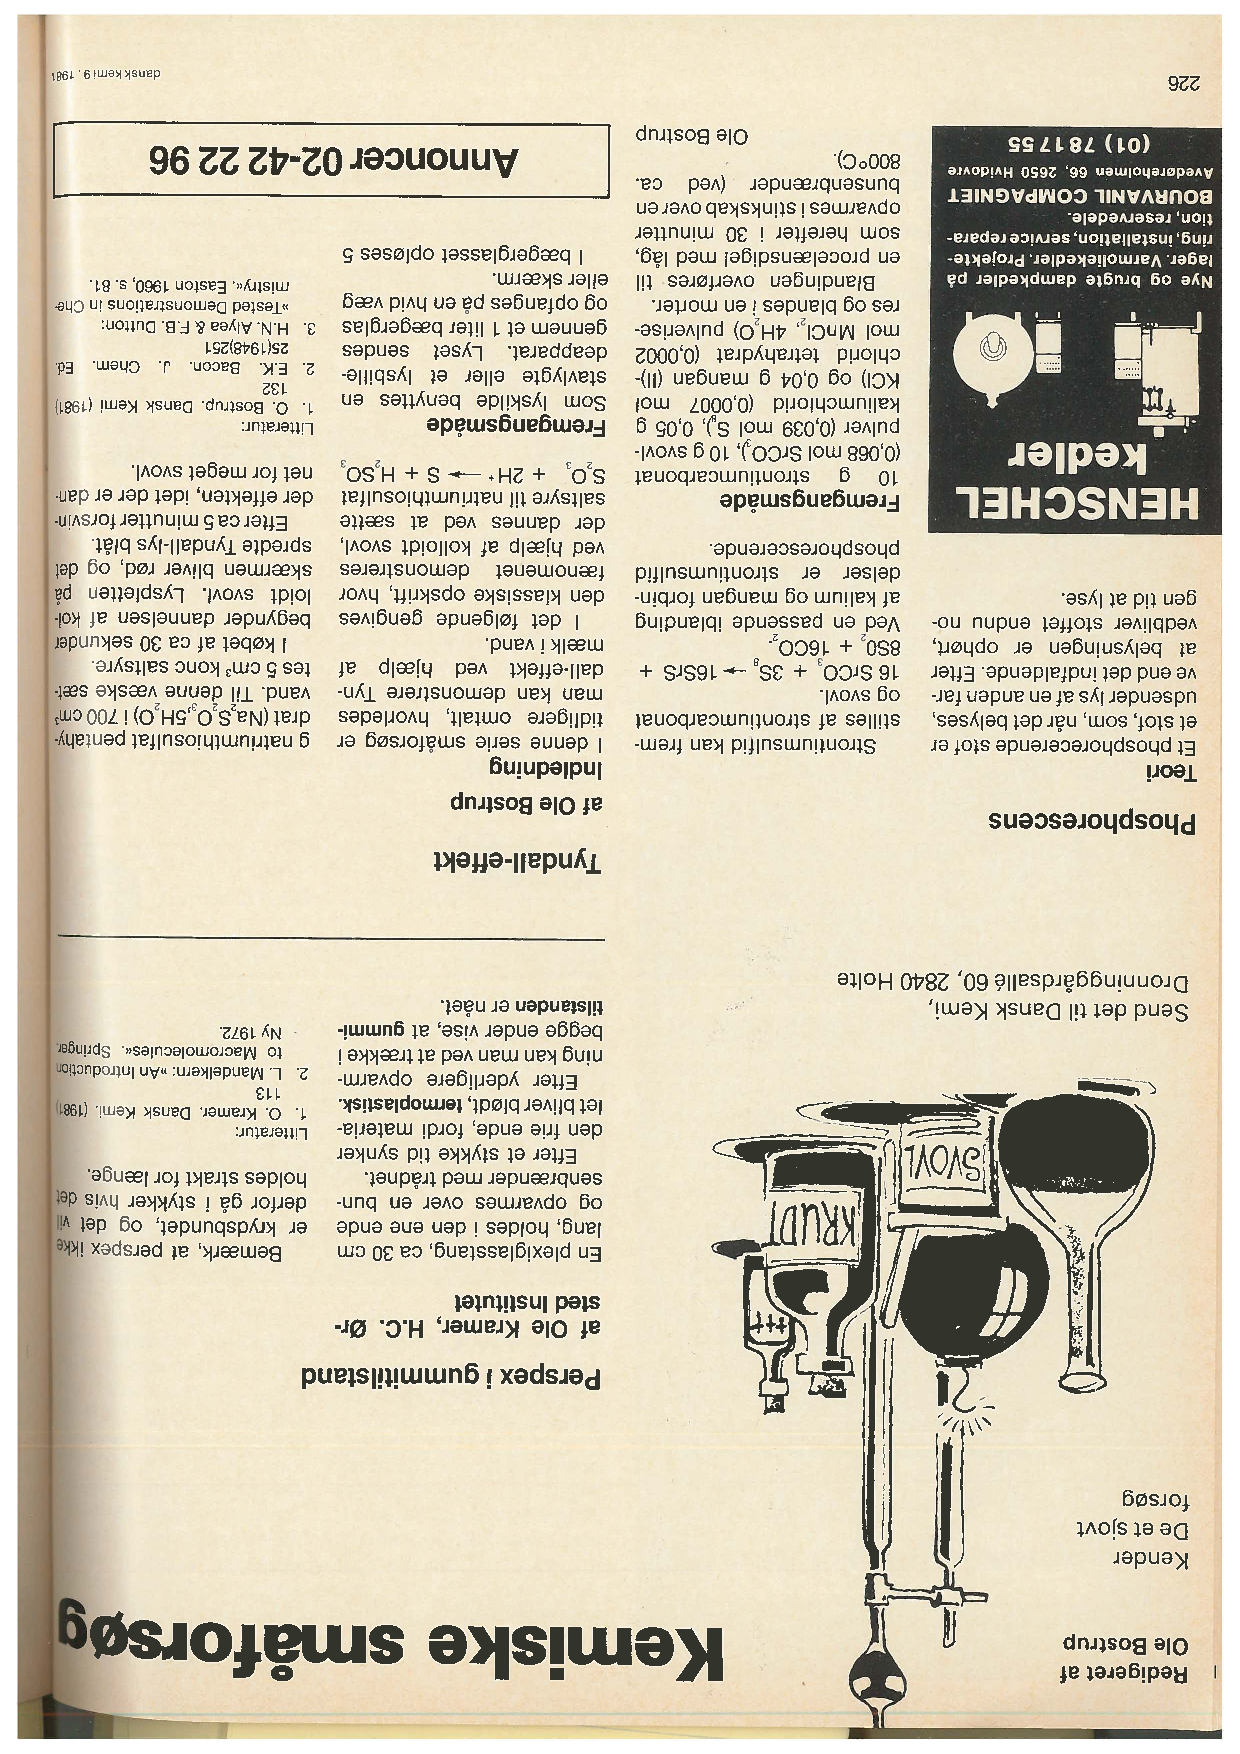
\includepdf[pages=-]{pdfs/1981-62-9-226.pdf}
\emne{Tyndall-effekt}
\danskkemi{Dansk Kemi 62, 9, 1981, p. 226}
\forfatter{Ole Bostrup}

\deloverskrift{Indledning}
I denne serie småforsøg er tidligere omtalt, hvorledes man kan
demonstrere Tyndall-effekt ved hjælp af mælk i vand.
I det følgende gengives den klassiske opskrift, hvor fænomenet
demonstreres ved hjælp af kolloidt svovl, der dannes ved at sætte
saltsyre til natriumthiosulfat
\ch{S2O3 + 2H+ -> S + H2SO3}

\deloverskrift{Fremgangsmåde}
Som lyskilde benyttes en stavlygte eller et lysbilledeapparat. Lyset
sendes gennem et 1 liter bægerglas og opfanges på en hvid væg eller
skærm.
I bægerglasset opløses 5 g natriumthiosulfat pentahydrat
(\ch{Na2S2O3 , 5 H2O}) i 700 cm3 vand. Til dene væske sættes 5 cm3
konc saltsyre.
I købet af ca 30 sekunder begynder dannelsen af kolloidt svovl.
Lyspletten på skærmen bliver rød, og det spredte Tyndall-lys blåt.
Efter ca 5 minutter forsvinder effekten, idet der er dannet for
meget svovl.

Litteratur:
1. O. Bostrup. Dansk Kemi (1981) 132
2. E.K. Bacon. J.Chem.Ed. 25(1948)251
3. H.N. Alyea \& F.B. Dutton: "Tested Demonstrations in Chemistry".
Easton 1960, s. 81.

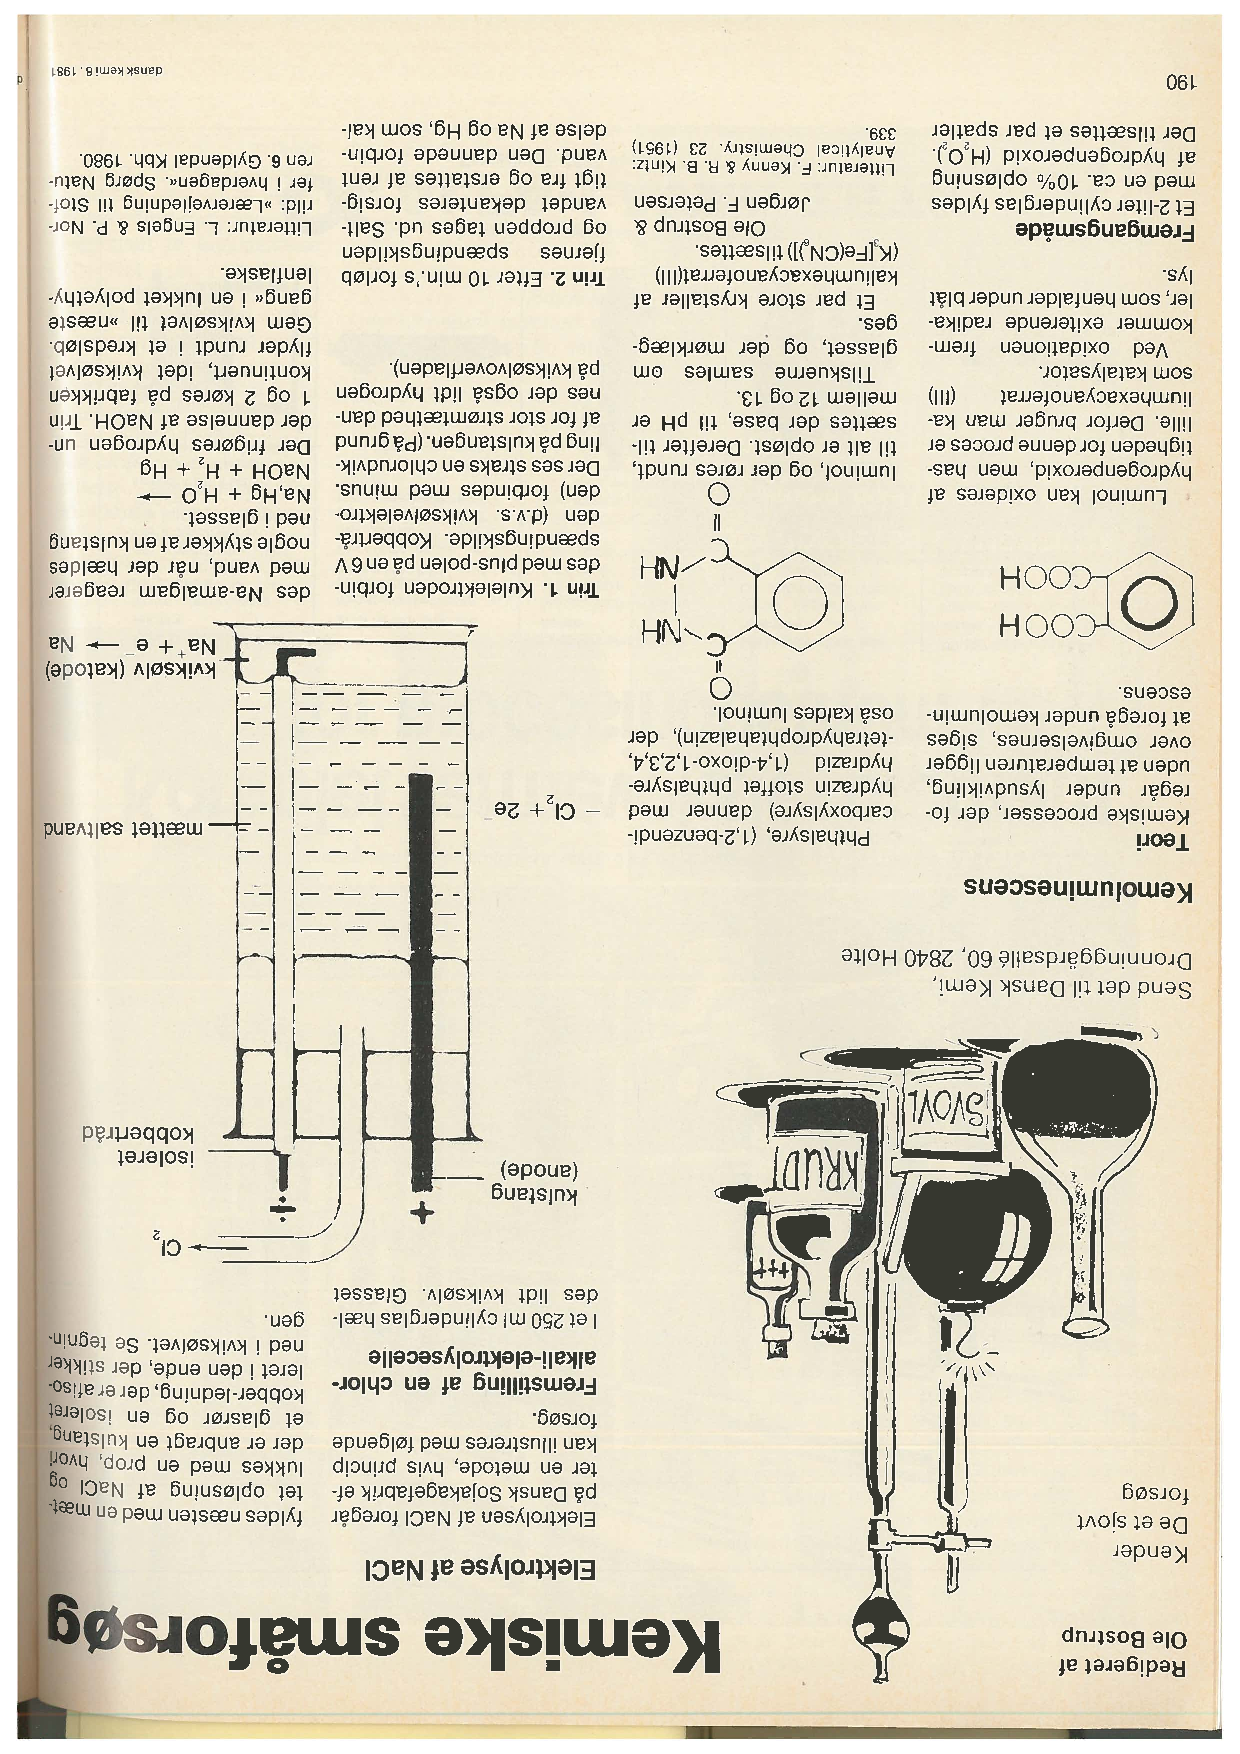
\includepdf[pages=-]{pdfs/1981-62-8-190.pdf}

\emne{Elektrolyse af NaCl}
\danskkemi{1981-62-8 190}
\forfatter{}

Elektrolysen af NaCl foregår på Dansk Sojakagefabrik efter en metode, hvis
princip kan illustreres med følgende forsøg.
\deloverskrift{Fremstilling af en chlor-alkali-elektrolysecelle.}
I et 250 ml cylinderglas hældes lidt kviksølv. Glasset fyldes næsten med en
mættet opløsning af NaCl og lukkes med en prop, hvori der er anbragt en
kulstang, et glasrør og en isoleret kobber-ledning, der er afisoleret i den
ende, der stikker ned i kviksølvet. Se tegningen.

OG HER SKAL VI SÅ HAVE INDSAT EN ILLUSTRATION

\deloverskrift{Trin 1.} Kulelektroden forbindes med plus-polen på en 6 V
spændingskilde.

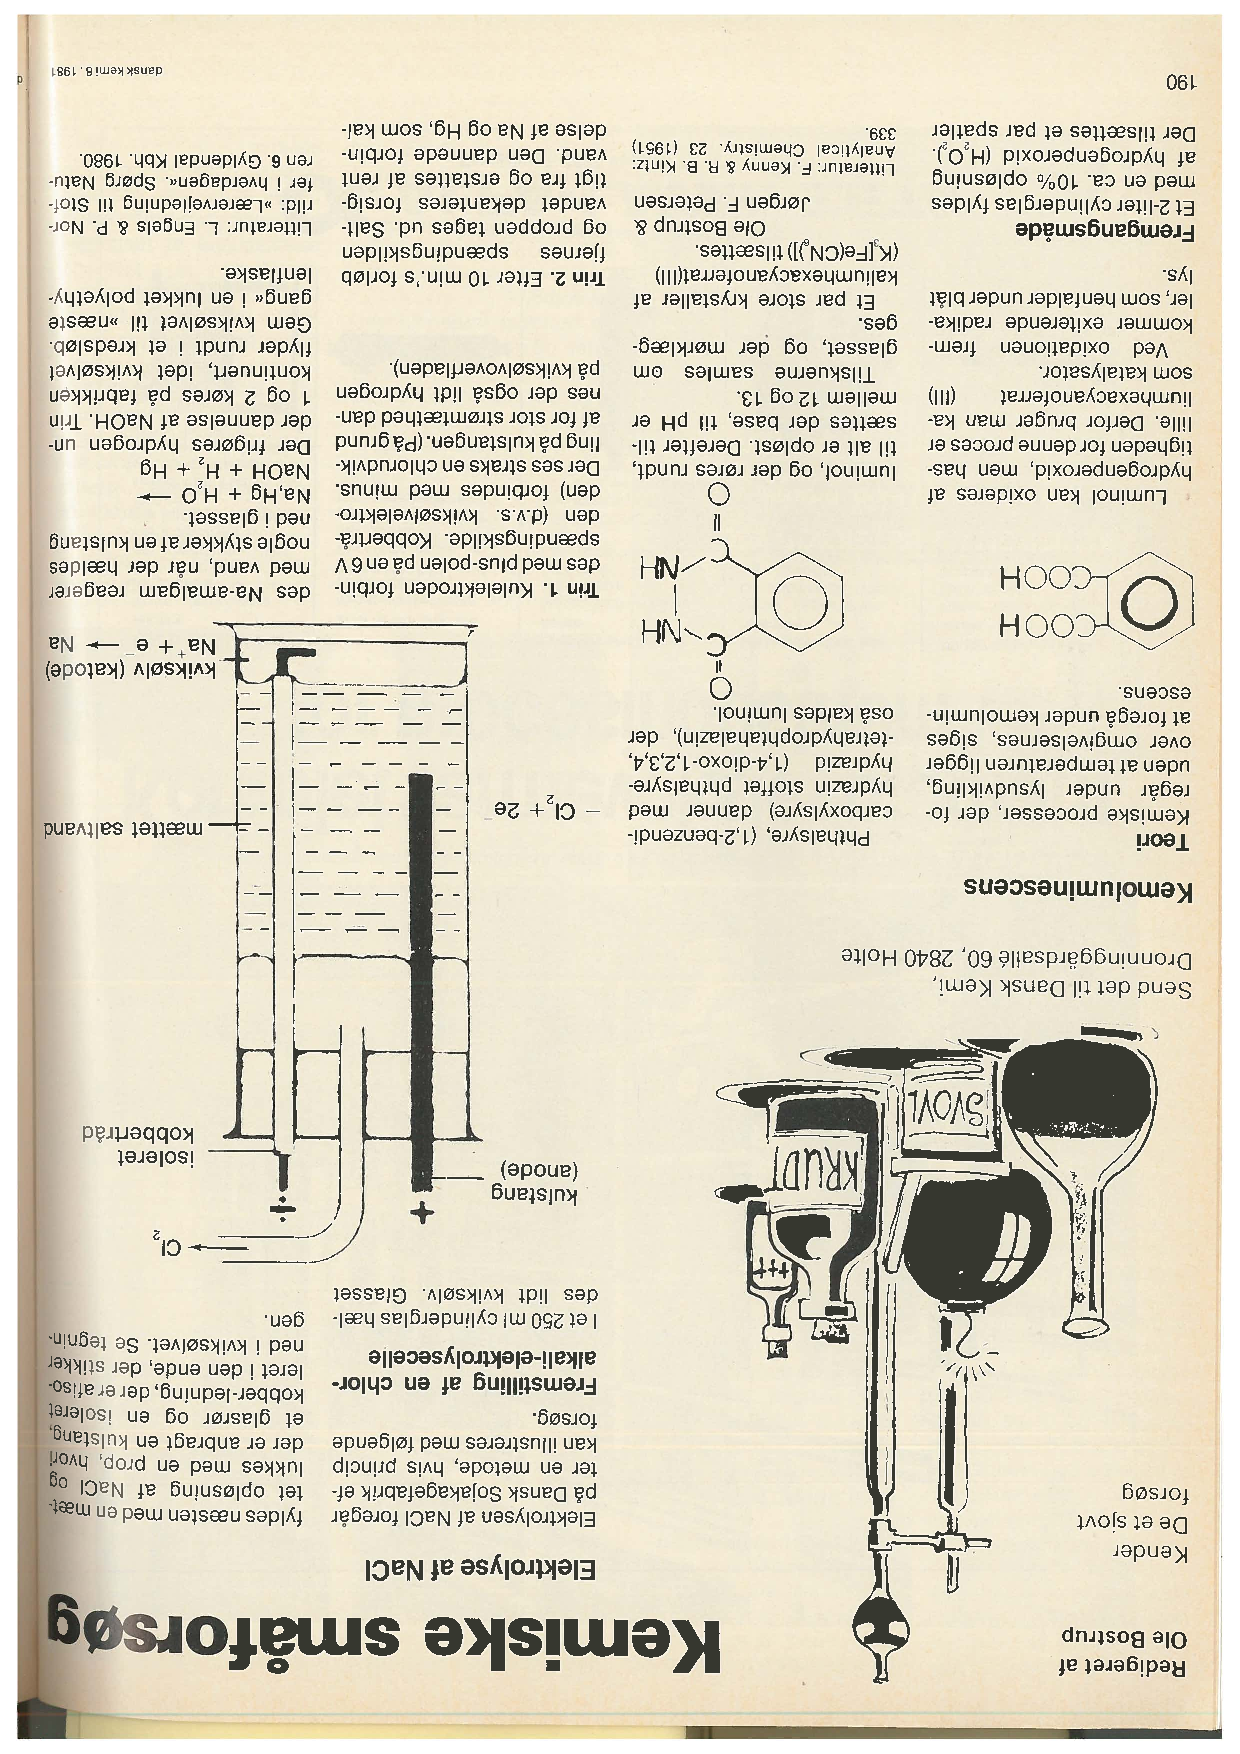
\includepdf[pages=-]{pdfs/1981-62-8-190.pdf}

\emne{}
\danskkemi{1981-62-8 192}
\forfatter{}
Ikke elektrolyse tingen.


\deloverskrift{}


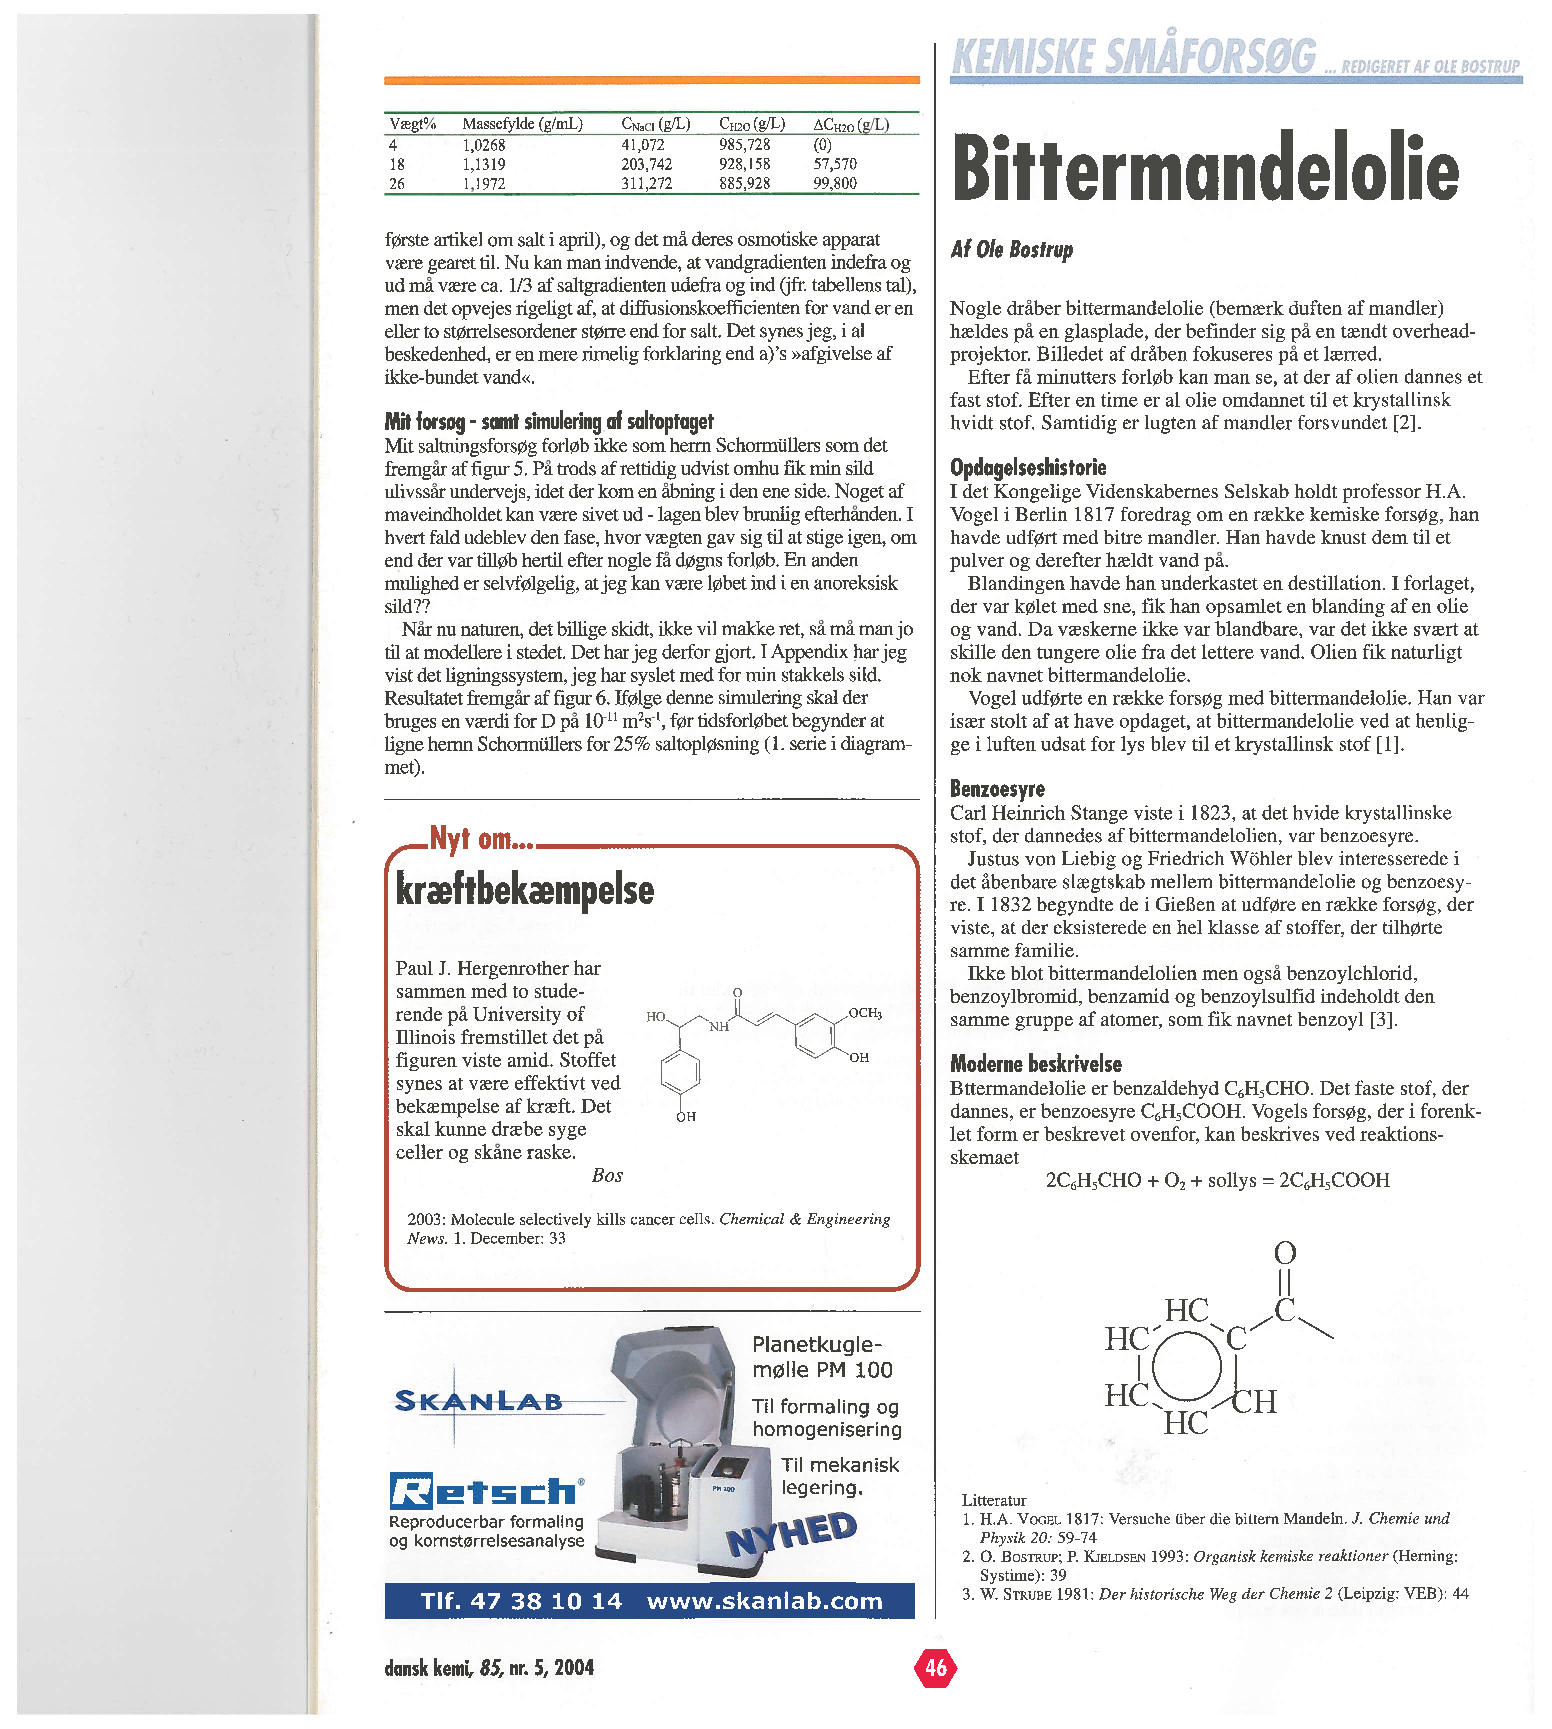
\includepdf[pages=-]{pdfs/2004-85-5-46.pdf}
\emne{Bittermandelolie}


\danskkemi{85 nr. 5, s. 46}

Nogle dråber bittermandelolie (bemærk duften af mandler) hældes på en glasplade, der befinder sig på en tændt overheadprojektor. Billedet af dråben fokuseres på et lærred.
Efter få minutters forløb kan man se, at der af olien dannes et fast stof. Efter en time er al olie omdannet til et krystallinsk hvidt stof. Samtidig er lugten af mandler forsvundet [2].

\deloverskrift{Opdagelseshistorie}

I det Kongelige Videnskabernes Selskab holdt professor H.A. Vogel i Berlin 1817 foredrag om en række kemiske forsøg, han havde udført med bitre mandler. Han havde knust dem til et pulver og derefter hældt vand på.
Blandingen havde han underkastet en destillation. I forlaget, der var kølet med sne, fik han opsamlet en blanding af en olie og vand. Da væskerne ikke var blandbare, var det ikkesvært at skille den tungere olie fra det lettere vand. Olien fik naturligt nok navnet bittermandelolie.
Vogel udførte en række forsøg med bittermandelolie. Han var især stolt af at have opdaget, at bittermandelolie ved at henligge i luften udsat for lys blev til et krystallinsk stof [1].

\deloverskrift{Benzoesyre}
Carl Heinrich Stange viste i 1823, at det hvide krystallinske stof, der dannedes af bittermandelolien, var benzoesyre.
Justus von Liebig og Friedrich Wöhler blev interesserede i det åbenbare slægtskab mellem bittermandelolie og benzoesyre. I 1832 begyndte de i Gießen at udføre en række forsøg, der viste, at der eksisterede en hel klasse af stoffer, der tilhørte samme familie.
Ikke blot bittermandelolien men også benzoylchlorid, benzoylbromid, benzamid og benzoylsulfid indeholdt den samme gruppe af atomer, som fik navnet benzoyl [3].

\deloverskrift{Moderne beskrivelse}
Bittermandelolie er benzaldehyd \ch{C6H5CHO}. Det faste stof, der dannes, er benzoesyre \ch{C6H5COOH}. Vogels forsøg, der i forenklet form er beskrevet ovenfor, kan beskrives ved reaktionsskemaet

\ch{2 C6H5CHO + O2 + sollys = 2 C6H5COOH}

\chemfig{
                   O% 8
            =[:270]% 7
                      (
                -[:330]% 9
                      )
            -[:210]% 3
            -[:270]% 2
            -[:210]% 1
                      (
    -[:90,,,,draw=none]\mcfcringle{1.3}% (o)
                      )
            -[:150]% 6
             -[:90]% 5
             -[:30]% 4
                      (
                -[:330]% -> 3
                      )
}

Litteratur
H.A. Vogel, 1817: Versuche über die bittern Mandeln. J.Chemie und Physik 20: 59-74
O.Bostrup, P.Kjeldsen 1993, Organisk kemiske reaktioner (Herning: Systime): 39
W. Strube 1981: Der historische Weg der Chemie 2 (Leipzib: VEB):44

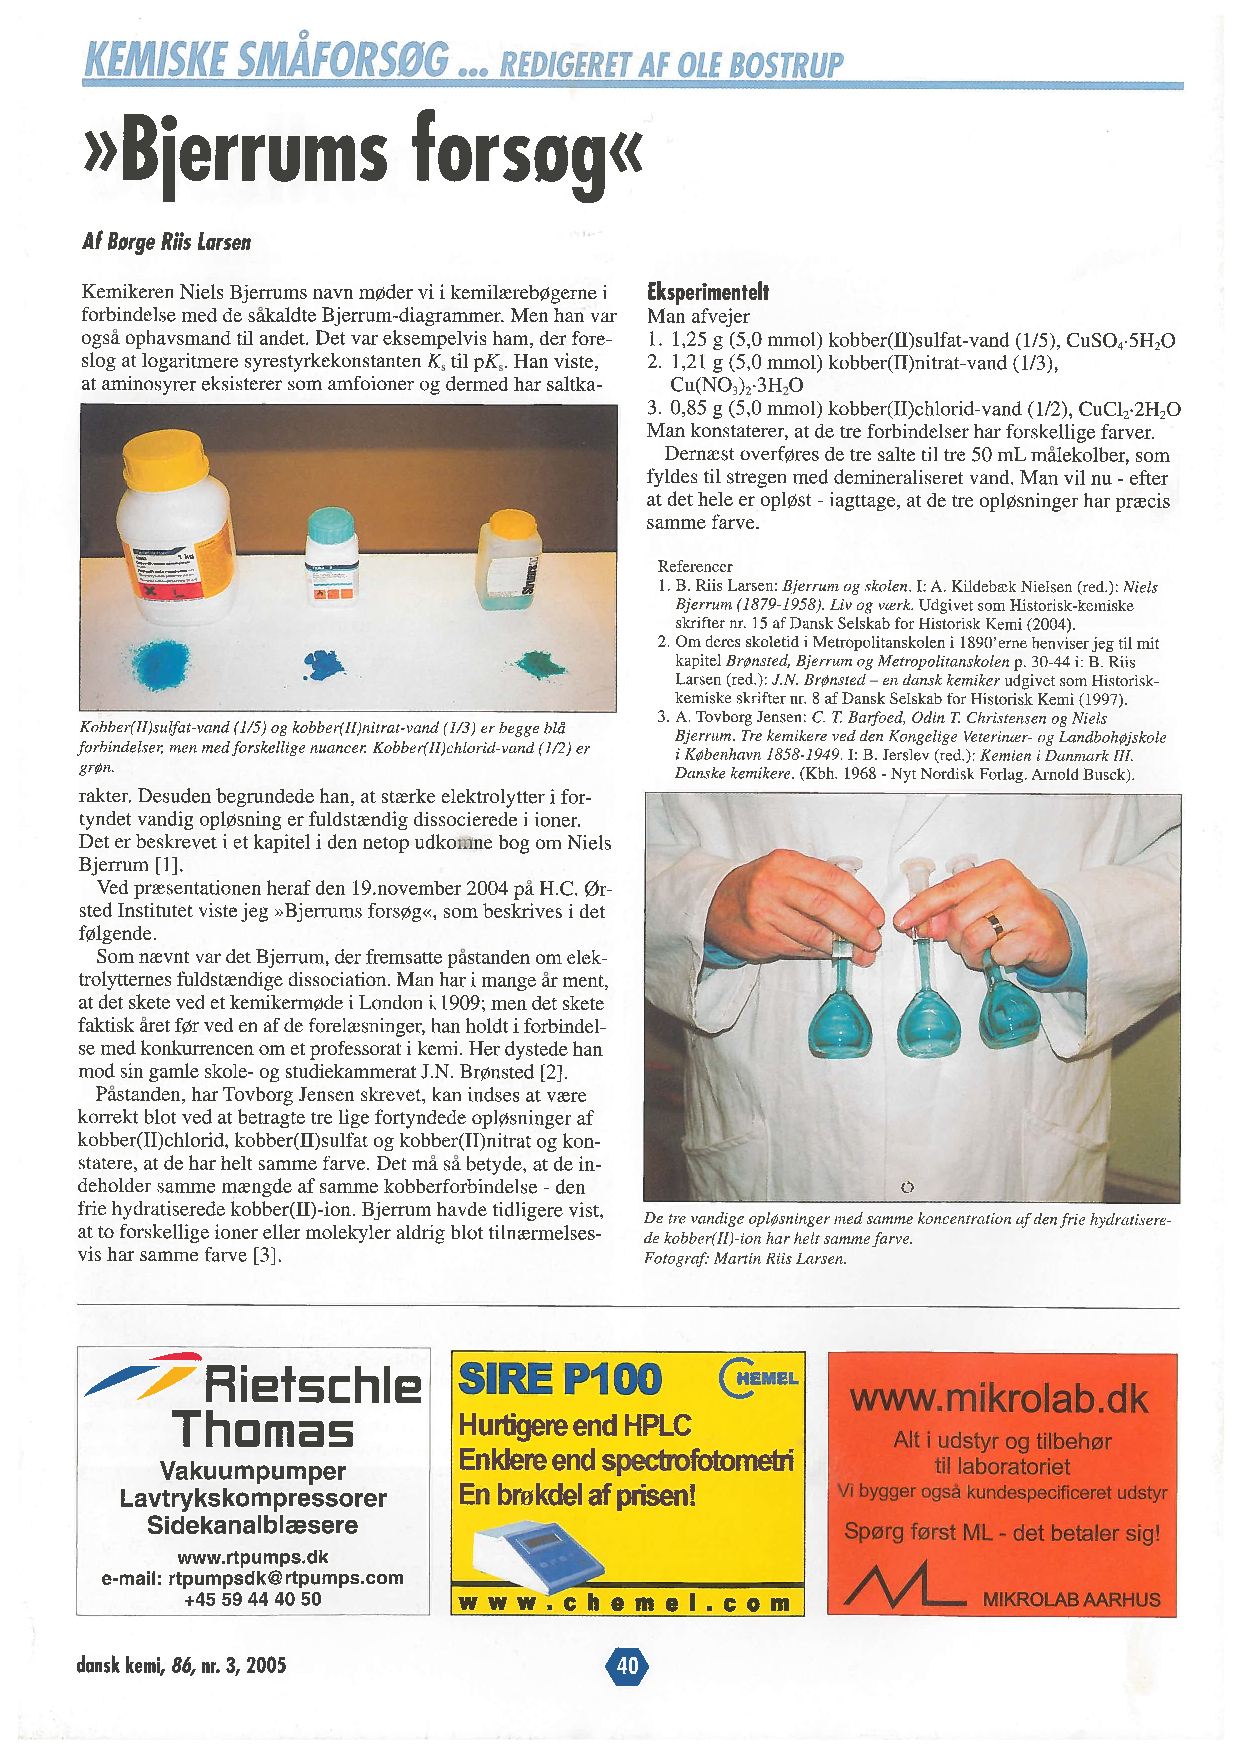
\includepdf[pages=-]{pdfs/2005-86-3-40.pdf}

\emne{"Bjerrums forsøg"}
\danskkemi{Dansk Kemi 86, 3, 2005, p. 40}

Af Børge Riis Larsen

Kemikeren Niels Bjerrums navn møder vi i kemilærebøgerne i forbindelse med de
såkaldte Bjerrum-diagrammer. Men han var også ophavsmand til andet. Det var
eksempelvis ham, der foreslog at logaritmere syrestyrkekonstanten $K_{s}$
til $pK_{s}$.
Han viste at aminosyrer eksisterer som amfoioner og dermed har saltkarakter.
Desuden begrundede han, at stærke elektrolytter i fortyndet vandig opløsning
er fuldstændig dissocierede i ioner. Det er beskrevet i et kapitel i den netop
udkomne bog om Niels Bjerrum [1].

Ved præsentationen heraf den 19. november 2004 på H.C. Ørsted Institutet viste
jeg "Bjerrums forsøg", som beskrives i det følgende.

Som nævnt var det Bjerrum, der fremsatte påstanden om elektrolytternes
fuldstændige dissociation. Man har i mange år ment, at det skete ved et
kemikermøde i London i 1909; men det skete faktisk året før ved en af de
forelæsninger, han holdt i forbindelse med konkurrencen om et professorat i
kemi. Her dystede han mod sin gamle skole- og studiekammerat J.N. Brønsted [2].

Påstanden, har Tovborg Jensen skrevet, kan indses at være korrekt blot ved at
betragte tre lige fortyndede opløsninger af kobber(II)chlorid, kobber(II)sulfat
og kobber(II)nitrat og konstatere, at de har helt samme farve. Det må så betyde,
at de indeholder samme mængde af samme kobberforbindelse - den frie hydratiserede
kobber(II)-ion. Bjerrum havde tidligere vist, at to forskellige ioner eller
molekyler aldrig blot tilnærmelsesvis har samme farve [3].


\deloverskrift{Eksperimentelt}


Man afvejer

1. 1,25 g (5,0 mmol) kobber(II)sulfat-vand (1/5), \ch{CuSO4}$\cdotp$\ch{5 H2O}

2. 1,21 g (5,0 mmol) kobber(II)nitrat-vand (1/3), \ch{Cu(NO3)2}$\cdotp$\ch{3 H2O}

3. 0.85 g (5,0 mmol) kobber(II)chlorid-vand (1/2), \ch{CuCl2}$\cdotp$\ch{2 H2O}

Man konstaterer, at de tre forbindelser har forskellige farver.

Dernæst overføres de tre salte til tre 50 mL målekolber, som fyldes til stregen
med demineraliseret vand. Man vil nu - efter at det hele er opløst - iagttage,
at de tre opløsninger har præcis samme farve.

Referencer
1. B. Riis Larsen: Bjerrum og skolen. I A. Kildebæk Nielsen (red.): Niels Bjerrum
(1879-1958). Liv og værk. Udgivet som Historisk-kemiske skrifter nr. 15 af Dansk
Selskab for Historisk Kemi (2004).
2. Om deres skoletid i Metropolitanskolen i 1890'erne henviser jeg til mit
kapitel Brønsted, Bjerrum og Metropolitanskolen p. 30-40 i: B. Riis Larsen (red.):
J.N. Brønsted - en dansk kemiker udgivet som Historisk-kemiske skrifter nr. 8
af Dansk Selskab for Historisk Kemi (1997).
3. A. Tovborg Jensen: C.T. Barfoed, Odin T. Christensen og Niels Bjerrum. Tre
kemikere ved den Kongelige Veterinær- og Landbohøjskole i København 1858-1949. I:
B. Jerslev (red.): Kemien i Danmark III. Danske Kemikere. (Kbh. 1968 - Nyt Nordisk
Forlag. Arnold Busck).

\include{dele/86-8}
%\includepdf[pages=-]{pdfs/.pdf}
\emne{Småforsøg med protolytiske reaktioner i vandige saltopløsninger}

\danskkemi{87 2 18 }

\deloverskrift{Saltes reaktion med vand.}


De anførte forsøg er en del af en samling, der blev udviklet under ledelse af R.W. Asmussen på Kemisk Laboratorium B på DTU i 1950'erne

Den protolytiske tilstand i opløsninger af salte er bestemt af de tilstedeværende ioners protolytiske karakter.

Ved brug af protolytiske indikatorer kan man danne sig et skøn over vandige saltopløsningers pH-værdi. De protolytiske indikatorer skifter farve i et for hver indikator karakteristisk område.


\deloverskrift{Forberedelse}

Ved forsøgene får man brug for

indikatorer: methylorange $\cdotp$ bromthymolblåt $\cdotp$ phenolphthalein

salte: jernalun $\cdotp$ aluminiumnitrat $\cdotp$ natriumchlorid
       natriumhydrogencarbonat $\cdotp$ natriumcarbonat
                                natriumsulfid



\deloverskrift{Fremgangsmåde}

Følgende opløsninger fremstilles:

1. 4 reagensglas fyldes halvt med vand, og 4-5 dråber methylorange tilsættes. Til hvert enkelt glas sættes hhv. én spatelfuld 1) jernalun, 2) aluminiumnitrat, 3) natriumhydrogencarbonat og 4) natriumchlorid.

2. Til 4 reagensglas med vand og 4-5 dråber bromthymolblåt sættes hhv. én spatelfuld 1) aluminiumnitrat, 2) natriumchlorid, 3) natriumhydrogencarbonat og 4) natriumcarbonat.

3. Til 4 reagensglas med vand og 4-5 dråber phenolphthalein sætets hhv. en spatelfuld 1) natriumchlorid, 2) natriumhydrogencarbonat, 3) natriumcarbonat og 4) natriumsulfid.



Litteratur

R.W. Asmussen m.fl. 1955: Vejledning til øvelser i Kemi for M, B og E. Polyteknisk Forening: 47.

%\includepdf[pages=-]{pdfs/.pdf}
\emne{Emil Petersen – og et småforsøg}


\danskkemi{Dansk Kemi 2006, 87(5) p 46}



»Kobbersulfat prøves for Jern; 2 Gr. opløses i Vand, der tilsættes lidt Salpetersyre og Opløsningen inddampes. Derefter overmættes den med Ammoniak og fi ltreres; et Indhold af Jern vil
da vise sig som en rødbrun Rest af Jerntveiltehydrat paa Filtret«.
Ovenstående småforsøg er beskrevet af Emil Petersen og offentliggjort i hans Titreranalytiske Methoder, der udkom i 1905.
Emil Petersen blev født den 12. april 1856. Han blev døbt
Christian Emil Ulrich Petersen, men undlod altid mellemnavnene og kaldte sig Emil Petersen – så det vil vi også gøre her.
Emil Petersen blev optaget på Den Polytekniske Læreanstalt
og bestod kandidateksamen i Anvendt Naturvidenskab i 1879.
Han var derefter en kort tid ansat ved Elghammars Järnvärk i
Småland, hvor han udarbejdede en metode til fremstilling af
vanadiumpræparater af slaggen fra malm fra Taberg. Han rejste
tilbage til Danmark og bestod studentereksamen i 1881. I 1888
blev han dr.phil. på afhandlingen Vanadinet og dets nærmeste
Analoger.

I 1870-1872 var han frivillig lærling i marinen, 1872-1874
elev på søofficersskolen. 1881-1882 assistent for S.M. Jørgensen
ved Kemisk Laboratorium på Den Polytekniske Læreanstalt og
1882-1883 i Paris, hvor han studerede naturvidenskabshistorie.

Efter hjemkomsten skrev han en artikelserie i »Tilskueren« om
franske naturvidenskabsmænd. 1885-1893 assistent ved Universitetets kemiske laboratorium, 1895-1901 docent og 1901-1907
professor samme sted.

Hans helbred var ikke godt: Den 2. juli 1907 døde han 51 år
gammel – alt for ung. Af mange historikere omtales han som
ham, der indførte Den Fysiske Kemi i Danmark.



\chapter{Diverse administrativt}
Skriftstørrelsen skal være 11.
Hvilken font? Vistnok Times Roman-font
Vi skal nok kigge på margener også.

Pakken chemformula giver adgang til:
\ch{3 H2O}

\ch{1/2 H2O}

\ch{AgCl2-}

\ch{H2_{(aq)}}

Se gerne https://tex.stackexchange.com/questions/384610/how-to-write-a-chemical-formula

Vi skal have separat sidenummerering på de første sider med små romertal. Og ingen sidenummerering på den allerførste side.

Der er rod med nogle af pdf'erne, der er vendt på hovedet. De kan vendes ved hjælp af programmet
 pdf mix tools.



\begin{longtable}{ |l|l|l|l|p{2.7cm}|l|p{2cm}| }
År & Vol & Iss & Side & PDF/Link & tex & Note \\
\hline
\endhead % all the lines above this will be repeated on every page
 2018 & 99 & 8     &      NA &  &  & \\
 2018 & 99 & 7     &      NA &  &  & \\
 2018 & 99 & 6     &      NA &  &  & \\
 2018 & 99 & 5     &      NA &  &  & \\
 2018 & 99 & 4     &      NA &  &  & \\
 2018 & 99 & 3     &      NA &  &  & \\
 2018 & 99 & 2     &      NA &  &  & \\
 2018 & 99 & 1     &      NA &  &  & \\
 2017 & 98 & 11/12 &      NA &  &  & \\
 2017 & 98 & 10    &      NA &  &  & \\
 2017 & 98 & 9     &      NA &  &  & \\
 2017 & 98 & 8     &      NA &  &  & \\
 2017 & 98 & 6/7   &      NA &  &  & \\
 2017 & 98 & 5     &      NA &  &  & \\
 2017 & 98 & 4     &      NA &  &  & \\
 2017 & 98 & 3     &      NA &  &  & \\
 2017 & 98 & 1/2   &      NA &  &  & \\
 2016 & 97 & 12    &      NA &  &  & \\
 2016 & 97 &    11 &      NA &  &  & \\
 2016 & 97 &    10 &      NA &  &  & \\
 2016 & 97 &     9 &      NA &  &  & \\
 2016 & 97 &     8 &      NA &  &  & \\
 2016 & 97 &   6/7 &      NA &  &  & \\
 2016 & 97 &     5 &      NA &  &  & \\
 2016 & 97 &     4 &      NA &  &  & \\
 2016 & 97 &     3 &      NA &  &  & \\
 2016 & 97 &   1/2 &      NA &  &  & \\
 2015 & 96 &    12 &      NA &  &  & \\
 2015 & 96 &    11 &      NA &  &  & \\
 2015 & 96 &    10 &      NA &  &  & \\
 2015 & 96 &     9 &      NA &  &  & \\
 2015 & 96 &     8 &      NA &  &  & \\
 2015 & 96 &   6/7 &      NA  &  &  & \\
 2015 & 96 &     5 &      NA &  &  & \\
 2015 & 96 &     4 &      NA &  &  & \\
 2015 & 96 &     3 &      NA &  &  & \\
 2015 & 96 &   1/2 &      NA &  &  & \\
 2014 & 95 &    12 &      NA &  &  & \\
 2014 & 95 &    11 &      NA &  &  & \\
 2014 & 95 &    10 &      NA &  &  & \\
 2014 & 95 &     9 &      NA &  &  & \\
 2014 & 95 &     8 &         &  &  & \\
 2014 & 95 &   6/7 &         &  &  & \\
 2014 & 95 &     5 &         &  &  & \\
 2014 & 95 &     4 &         &  &  & \\
 2014 & 95 &     3 &         &  &  & \\
 2014 & 95 &   1/2 &         &  &  & \\
 2013 & 94 &    12 &         &  &   & \\
 2013 & 94 &    11 &         &  &  & \\
 2013 & 94 &    10 &         &  &  & \\
 2013 & 94 &     9 &         &  &  & \\
 2013 & 94 &     8 &         &  &  & \\
 2013 & 94 &   6/7 &         &  &  & \\
 2013 & 94 &     5 &         &  &  & \\
 2013 & 94 &     4 &         &  &  & \\
 2013 & 94 & 3 sup &         &  &  & \\
 2013 & 94 &     3 &         &  &  & \\
 2013 & 94 &   1/2 &         &  &  & \\
 2012 & 93 &    12 &         &  &  & \\
 2012 & 93 & 11 tl &         &  &  & \\
 2012 & 93 & 11    &         &  &  & \\
 2012 & 93 & 10    &         &  &   & \\
 2012 & 93 & 8     &         &  &  & \\
 2012 & 93 & 9     &         &  &  & \\
 2012 & 93 &   6/7 &         &  &  & \\
 2012 & 93 &     5 &         &  &  & \\
 2012 & 93 &     4 &         &  &  & \\
 2012 & 93 &     3 &         &  &  & \\
 2012 & 93 & 1/2tll&         &  &  & \\
 2012 & 93 &   1/2 &         &  &  & \\
 2011 & 92 &    12 &         &  &  & \\
 2011 & 92 &    11 &         &  &  & \\
 2011 & 92 &    10 &         &  &  & \\
 2011 & 92 &     9 &         &  &  & \\
 2011 & 92 &     8 &         &  &  & \\
 2011 & 92 &   6/7 &         &  &  & \\
 2011 & 92 &     5 &         &  &  & \\
 2011 & 92 &     4 &         &  &  & \\
 2011 & 92 &     3 &         &  &  & \\
 2011 & 92 &   1/2 &         &  &  & \\
 2010 & 91 &   12  &      NA &  &  & \\
 2010 & 91 &    11 &      NA &  &  & \\
 2010 & 91 &    10 &      NA &  &  & \\
 2010 & 91 &     9 &         &  &  & \\
 2010 & 91 &     8 &         &  &  & \\
 2010 & 91 &   6/7 &         &  &  & \\
 2010 & 91 &     5 &     NA  &  &  & \\
 2010 & 91 &     4 &     NA  &  &  & \\
 2010 & 91 &     3 &         &  &  & \\
 2010 & 91 &   1/2 &      NA &  &  & \\
 2009 & 90 &    12 &      NA &  &  & \\
 2009 & 90 &    11 &      NA &  &  & \\
 2009 & 90 &    10 &      NA &  &  & \\
 2009 & 90 &     9 &      NA &  &  & \\
 2009 & 90 &     8 &      NA &  &  & \\
 2009 & 90 &   6/7 &      NA &  &  & \\
 2009 & 90 &     5 &      NA &  &  & \\
 2009 & 90 &     4 &      NA &  &  & \\
 2009 & 90 &     3 &      NA &  &  & \\
 2009 & 90 &     2 &      NA &  &  & \\
 2009 & 90 &     1 &         &  &  & \\
 2008 & 89 &    12 &      NA &  &  & \\
 2008 & 89 &    11 &         &  &  & \\
 2008 & 89 &    10 &      NA &  &  & \\
 2008 & 89 &     9 &      NA &  &  & \\
 2008 & 89 &     8 &      NA &  &  & \\
 2008 & 89 &   6/7 &      NA &  &  & \\
 2008 & 89 &     5 &      NA &  &  & \\
 2008 & 89 &     4 &      NA &  &  & \\
 2008 & 89 &     3 &      NA &  &  & \\
 2008 & 89 &     2 &      NA &  &  & \\
 2008 & 89 &     1 &      NA &  &  & \\
 2007 & 88 &    12 &      NA &  &  & \\
 2007 & 88 &    11 &      NA &  &  & \\
 2007 & 88 &    10 &      NA &  &  & \\
 2007 & 88 &     9 &      NA &  &  & \\
 2007 & 88 &     8 &      NA &  &  & \\
 2007 & 88 &   6/7 &      NA &  &  & \\
 2007 & 88 &     5 &      NA &  &  & \\
 2007 & 88 &     4 &      NA &  &  & \\
 2007 & 88 &     3 &      NA &  &  & \\
 2007 & 88 &     2 &      NA &  &  & \\
 2007 & 88 &     1 &      NA &  &  & \\
 2006 & 87 &    12 &      NA &  &  & \\
 2006 & 87 &    11 &      NA &  &  & \\
 2006 & 87 &    10 &      NA &  &  & \\
 2006 & 87 &     9 &      65 & online &  & \\
 2006 & 87 &     8 &      31 & online &  & \\
 2006 & 87 &   6/7 &      NA &  &  & \\
 2006 & 87 &     5 &      46 & online &  & \\
 2006 & 87 &     4 &      NA &  &  & \\
 2006 & 87 &     3 &      38 & 2006-87-3-38 &  & \\
 2006 & 87 &     2 &      18 & online & 87-2  & \\
 2006 & 87 &     1 &      38 & 2006-87-1-38 &  & \\
 2005 & 86 &    12 &      32 & 2005-86-12-32 &  & \\
 2005 & 86 &    11 &      NA &  &  & \\
 2005 & 86 &    10 &      NA &  &  & \\
 2005 & 86 &     9 &         &  &  & \\
 2005 & 86 &     8 &      37 & 2005-86-8-37 & 86-8  & \\
 2005 & 86 &   6/7 &      39 &  &  & \\
 2005 & 86 &     5 &         &  &  & \\
 2005 & 86 &     4 &         & &  & \\
 2005 & 86 &     3 &      40 &  2005-86-3-40 & 86-3 & \\
 2005 & 86 &     2 &         &  &  & \\
 2005 & 86 &     1 &         &  &  & \\
 2004 & 85 &    12 &         &  &  & \\
 2004 & 85 &    11 &         &  &  & \\
 2004 & 85 &    10 &      NA &  &  & \\
 2004 & 85 &     9 &      54 &  &  & \\
 2004 & 85 &     8 &      39 &  &  & \\
 2004 & 85 &   6/7 &      NA &  &  & \\
 2004 & 85 &     5 &      46 & 2005-85-5-46 & 85-5 & \\
 2004 & 85 &     4 &      NA &  &  & \\
 2004 & 85 &     3 &      40 &  &  & \\
 2004 & 85 &     2 &      27 &  &  & \\
 2004 & 85 &     1 &         &  &  & \\
 2003 & 84 &    12 &         &  &  & \\
 2003 & 84 &    11 &         &  &  & \\
 2003 & 84 &    10 &         &  &  & \\
 2003 & 84 &     9 &         &  &  & \\
 2003 & 84 &     8 &         &  &  & \\
 2003 & 84 &   6/7 &         &  &  & \\
 2003 & 84 &     5 &         &  &  & \\
 2003 & 84 &     4 &         &  &  & \\
 2003 & 84 &     3 &         &  &  & \\
 2003 & 84 &     2 &         &  &  & \\
 2003 & 84 &     1 &     NA  &  &  & \\
 2002 & 83 &    12 &         &  &  & \\
 2002 & 83 &    11 &         &  &  & \\
 2002 & 83 &    10 &         &  &  & \\
 2002 & 83 &     9 &         &  &  & \\
 2002 & 83 &     8 &         &  &  & \\
 2002 & 83 &   6/7 &         &  &  & \\
 2002 & 83 &    5s &         &  &  & \\
 2002 & 83 &     5 &         &  &  & \\
 2002 & 83 &     4 &         &  &  & \\
 2002 & 83 &     3 &         &  &  & \\
 2002 & 83 &     2 &         &  &  & \\
 2002 & 83 &     1 &         &  &  & \\
 2001 & 82 &    12 &         &  &  & \\
 2001 & 82 &    11 &         &  &  & \\
 2001 & 82 &    10 &      NA &  &  & \\
 2001 & 82 &    9t &         &  &  & \\
 2001 & 82 &     9 &         &  &  & \\
 2001 & 82 &     8 &         &  &  & \\
 2001 & 82 &   6/7 &         &  &  & \\
 2001 & 82 &    5t &         &  &  & \\
 2001 & 82 &     5 &         &  &  & \\
 2001 & 82 &     4 &         &  &  & \\
 2001 & 82 &    3t &     NA  &  &  & \\
 2001 & 82 &     3 &         &  &  & \\
 2001 & 82 &     2 &         &  &  & \\
 2001 & 82 &     1 &         &  &  & \\
 2000 & 81 &    12 &         &  &  & \\
 2000 & 81 &    11 &         &  &  & \\
 2000 & 81 &    10 &         &  &  & \\
 2000 & 81 &    9t &         &  &  & \\
 2000 & 81 &     9 &         &  &  & \\
 2000 & 81 &     8 &         &  &  & \\
 2000 & 81 &   6/7 &     NA  &  &  & \\
 2000 & 81 &     5 &         &  &  & \\
 2000 & 81 &    4t &         &  &  & \\
 2000 & 81 &     4 &     NA  &  &  & \\
 2000 & 81 &    3t &         &  &  & \\
 2000 & 81 &     3 &         &  &  & \\
 2000 & 81 &     2 &         &    &  & \\
 2000 & 81 &     1 &         &  &  & \\
 1999 & 80 &    12 &         &  &  & \\
 1999 & 80 &    11 &         &  &  & \\
 1999 & 80 &    10 &         &  &  & \\
 1999 & 80 &     9 &     NA  &  &  & \\
 1999 & 80 &     8 &         &  &  & \\
 1999 & 80 &   6/7 &         &  &  & \\
 1999 & 80 &     5 &         &  &  & \\
 1999 & 80 &     4 &         &  &  & \\
 1999 & 80 &     3 &         &  &  & \\
 1999 & 80 &     2 &         &  &  & \\
 1999 & 80 &     1 &         &  &  & \\
 1998 & 79 &    12 &         &  &  & \\
 1998 & 79 &    11 &         &  &  & \\
 1998 & 79 &    10 &         &  &  & \\
 1998 & 79 &    9t &         &  &  & \\
 1998 & 79 &     9 &         &  &  & \\
 1998 & 79 &     8 &         &  &  & \\
 1998 & 79 &   6/7 &         &  &  & \\
 1998 & 79 &     5 &         &  &  & \\
 1998 & 79 &     4 &     NA  &  &  & \\
 1998 & 79 &     3 &         &  &  & \\
 1998 & 79 &     2 &     NA  &  &  & \\
 1998 & 79 &     1 &     NA  &  &  & \\
 1997 & 78 &    12 &         &  &  & \\
 1997 & 78 &    11 &         &  &  & \\
 1997 & 78 &    10 &         &  &  & \\
 1997 & 78 &     9 &         &  &  & \\
 1997 & 78 &     8 &         &  &  & \\
 1997 & 78 &   6/7 &         &  &  & \\
 1997 & 78 &     5 &     NA  &  &  & \\
 1997 & 78 &     4 &         &  &  & \\
 1997 & 78 &     3 &         &  &  & \\
 1997 & 78 &     2 &         &  &  & \\
 1997 & 78 &     1 &         &                &  & \\
 1996 & 77 &    12 &         &                &  & \\
 1996 & 77 &    11 &         &                &  & \\
 1996 & 77 &    10 &         &                &  & \\
 1996 & 77 &     9 &         &                &  & \\
 1996 & 77 &     8 &         &                &  & \\
 1996 & 77 &   6/7 &         &                &  & \\
 1996 & 77 &     5 &         &                &  & \\
 1996 & 77 &     4 &         &                &  & \\
 1996 & 77 &     3 &         &                &  & \\
 1996 & 77 &     2 &         &                &  & \\
 1996 & 77 &     1 &     NA  &                &  & \\
 1995 & 76 &    12 &         &                &  & \\
 1995 & 76 &    11 &         &                &  & \\
 1995 & 76 &    10 &         &                &  & \\
 1995 & 76 &     9 &         &                &  & \\
 1995 & 76 &     8 &         &                &  & \\
 1995 & 76 &   6/7 &         &                &  & \\
 1995 & 76 &     5 &         &                &  & \\
 1995 & 76 &     4 &         &                &  & \\
 1995 & 76 &     3 &         &                &  & \\
 1995 & 76 &     2 &         &                &  & \\
 1995 & 76 &     1 &         &                &  & \\
 1994 & 75 &    12 &         &                &  & \\
 1994 & 75 &    11 &         &                &  & \\
 1994 & 75 &    10 &         &                &  & \\
 1994 & 75 &     9 &         &                &  & \\
 1994 & 75 &     8 &         &                &  & \\
 1994 & 75 &   6/7 &         &                &  & \\
 1994 & 75 &     5 &         &                &   & \\
 1994 & 75 &     4 &         &                &  & \\
 1994 & 75 &     3 &         &                &  & \\
 1994 & 75 &     2 &         &                &  & \\
 1994 & 75 &     1 &         &                &  & \\
 1993 & 74 &    12 &         &                &  & \\
 1993 & 74 &    11 &         &                &  & \\
 1993 & 74 &    10 &         &                &  & \\
 1993 & 74 &     9 &         &                &  & \\
 1993 & 74 &     8 &         &                &  & \\
 1993 & 74 &   6/7 &         &                &  & \\
 1993 & 74 &     5 &         &                &  & \\
 1993 & 74 &     4 &         &                &  & \\
 1993 & 74 &     3 &         &                &  & \\
 1993 & 74 &     2 &         &                &  & \\
 1993 & 74 &     1 &         &                &  & \\
 1993 & 74 &   reg &         &                &  & \\
 1992 & 73 &    12 &         &                &  & \\
 1992 & 73 &    11 &         &                &  & \\
 1992 & 73 &    10 &         &                &  & \\
 1992 & 73 &     9 &         &                &  & \\
 1992 & 73 &     8 &         &                &  & \\
 1992 & 73 &   6/7 &         &                &  & \\
 1992 & 73 &     5 &         &                &  & \\
 1992 & 73 &     4 &         &                &  & \\
 1992 & 73 &     3 &         &                &  & \\
 1992 & 73 &     2 &         &                &  & \\
 1992 & 73 &     1 &         &                &  & \\
 1991 & 72 &    12 &         &                &  & \\
 1991 & 72 &    11 &         &                &  & \\
 1991 & 72 &    10 &         &                &  & \\
 1991 & 72 &     9 &         &                &  & \\
 1991 & 72 &     8 &         &                &  & \\
 1991 & 72 &   6/7 &         &                &  & \\
 1991 & 72 &     5 &         &                &  & \\
 1991 & 72 &     4 &         &                &  & \\
 1991 & 72 &     3 &         &                &  & \\
 1991 & 72 &     2 &         &                &  & \\
 1991 & 72 &     1 &         &                &  & \\
 1990 & 71 &    12 &         &                &  & \\
 1990 & 71 &    11 &         &                &  & \\
 1990 & 71 &    10 &         &                &  & \\
 1990 & 71 &     9 &         &                &  & \\
 1990 & 71 &     8 &         &                &  & \\
 1990 & 71 &   6/7 &         &                &  & \\
 1990 & 71 &     5 &         &                &   & \\
 1990 & 71 &     4 &         &                &  & \\
 1990 & ?  &     3 &         &                &  & \\
 1990 & ?  &     2 &         &                &  & \\
 1990 & ?  &     1 &         &                &  & \\
 1989 & 70 &    12 &         &                &   & \\
 1989 & 70 &    11 &         &                &  & \\
 1989 & 70 &    10 &         &                &  & \\
 1989 & 70 &     9 &         &                &  & \\
 1989 & 70 &     8 &         &                &  & \\
 1989 & 70 &   6/7 &         &                &  & \\
 1989 & 70 &     5 &         &                &  & \\
 1989 & 70 &     4 &         &                &  & \\
 1989 & 70 &     3 &         &                &  & \\
 1989 & 70 &     2 &         &                &  & \\
 1989 & 70 &     1 &         &                &  & \\
 1988 & 69 &    12 &         &                &  & \\
 1988 & 69 &    11 &         &                &  & \\
 1988 & 69 &    10 &         &                &  & \\
 1988 & 69 &     9 &         &                &  & \\
 1988 & 69 &     8 &         &                &  & \\
 1988 & 69 &   6/7 &         &                &  & \\
 1988 & 69 &     5 &         &                &  & \\
 1988 & 69 &     4 &         &                &  & \\
 1988 & 69 &     3 &         &                &  & \\
 1988 & 69 &     2 &         &                &  & \\
 1988 & 69 &     1 &         &                &  & \\
 1987 & 68 &    12 &         &                &  & \\
 1987 & 68 &    11 &         &                &  & \\
 1987 & 68 &    10 &         &                &  & \\
 1987 & 68 &     9 &         &                &  & \\
 1987 & 68 &     8 &         &                &  & \\
 1987 & 68 &   6/7 &         &                &  & \\
 1987 & 68 &     5 &         &                &  & \\
 1987 & 68 &     4 &         &                &  & \\
 1987 & 68 &     3 &         &                &  & \\
 1987 & 68 &     2 &         &                &  & \\
 1987 & 68 &     1 &         &                &  & \\
 1986 & 67 &    12 &         &                &  & \\
 1986 & 67 &    11 &         &                &  & \\
 1986 & 67 &    10 &         &                &  & \\
 1986 & 67 &     9 &         &                &  & \\
 1986 & 67 &     8 &         &                &  & \\
 1986 & 67 &   6/7 &         &                &  & \\
 1986 & 67 &     5 &         &                &  & \\
 1986 & 67 &     4 &         &                &  & \\
 1986 & 67 &     3 &         &                &  & \\
 1986 & 67 &     2 &         &                &  & \\
 1986 & 67 &     1 &         &                &  & \\
 1985 & 66 &    12 &         &                &  & \\
 1985 & 66 &    11 &         &                &  & \\
 1985 & 66 &    10 &         &                &  & \\
 1985 & 66 &     9 &         &                &  & \\
 1985 & 66 &     8 &         &                &  & \\
 1985 & 66 &   6/7 &         &                &  & \\
 1985 & 66 &     5 &         &                &  & \\
 1985 & 66 &     4 &         &                &  & \\
 1985 & 66 &     3 &         &                &  & \\
 1985 & 66 &     2 &         &                &  & \\
 1985 & 66 &     1 &         &                &  & \\
 1984 & 65 &    12 &         &                &  & \\
 1984 & 65 &    11 &         &                &  & \\
 1984 & 65 &    10 &     282 & 1984-65-10-282 &  & \\
 1984 & 65 &     9 &         &                &  & \\
 1984 & 65 &     8 &         &                &  & \\
 1984 & 65 &   6/7 &         &                &  & \\
 1984 & 65 &     5 &         &                &  & \\
 1984 & 65 &     4 &         &                &  & \\
 1984 & 65 &     3 &         &                &  & \\
 1984 & 65 &     2 &         &                &  & \\
 1984 & 65 &     1 &         &                &  & \\
 1983 & 64 &    12 &         &                &  & \\
 1983 & 64 &    11 &         &                &  & \\
 1983 & 64 &    10 &         &                &  & \\
 1983 & 64 &     9 &         &                &  & \\
 1983 & 64 &     8 &         &                &  & \\
 1983 & 64 &   6/7 &         &                &  & \\
 1983 & 64 &     5 &         &                &  & \\
 1983 & 64 &     4 &         &                &  & \\
 1983 & 64 &     3 &         &                &  & \\
 1983 & 64 &     2 &         &                &  & \\
 1983 & 64 &     1 &         &                &  & \\
 1982 & 63 &    12 &         &                &  & \\
 1982 & 63 &    11 &         &                &  & \\
 1982 & 63 &    10 &         &                &  & \\
 1982 & 63 &     9 &         &                &  & \\
 1982 & 63 &     8 &         &                &  & \\
 1982 & 63 &   6/7 &         &                &  & \\
 1982 & 63 &     5 &         &                &  & \\
 1982 & 63 &     4 &         &                &  & \\
 1982 & 63 &     3 &         &                &  & \\
 1982 & 63 &     2 &         &                &  & \\
 1982 & 63 &     1 &         &                &  & \\
 1982 & 63 &   6/7 &         &                &  & ??? sidetal er mærkelige \\
 1981 & 62 &     1 &      24 &   1981-62-1-24 &  & \\
 1981 & 62 &     2 &   42-43 & 1981-62-2-42, 1981-62-2-43 &  & \\
 1981 & 62 &     3 &   70-71 & 1981-62-3-70, 1981-62-3-71 & 62-3-a & \\
 1981 & 62 &   3 &   70-71 & 1981-62-3-70, 1981-62-3-71 &  & Flere forsøg \\
 1981 & 62 &     4 &     113 &  1981-62-4-113 &  & \\
 1981 & 62 &     5 &     132 &  1981-62-5-132 &  & \\
 1981 & 62 &   6/7 &     168 & 1981-62-67-168 &  & \\
 1981 & 62 &     8 &     190 &  1981-62-8-190 & 62-8-a & \\
 1981 & 62 &     8 &     190 &  1981-62-8-190 & 62-8-b & \\
 1981 & 62 &     9 &     226 &  1981-62-9-226 &  62-9-a & Der er flere \\
 1981 & 62 &     9 &     226 &  1981-62-9-226 &  62-9-b & Der er flere \\
 1981 & 62 &     9 &     226 &  1981-62-9-226 &  62-9-c & Der er flere \\
 1981 & 62 &    10 & 240-241 & 1981-62-10-240, 1981-62-10-241 &  & \\
 1981 & 62 &    11 &     278 & 1981-62-11-278 &  & \\
 1981 & 62 &    12 &     320 & 1981-62-12-320 &  & \\
 1980 & 61 &     1 &      34 &   1980-61-1-34 & 61-1 & \\
 1980 & 61 &     2 &      62 &   1980-61-2-62 & 61-2-a & \\
 1980 & 61 &     2 &      62 &   1980-61-2-62 & 61-2-b & \\
 1980 & 61 &     3 &      86 &   1980-61-3-86 &  & \\
 1980 & 61 &     4 &      NA &    NA          &  & \\
 1980 & 61 &     5 &     154 & 1980-61-5-154  &  & \\
 1980 & 61 &   6/7 &     174 & 1980-61-67-173, 1980-61-67-174 &  & \\
 1980 & 61 &     8 &    192f & 1980-61-8-192, 1980-61-8-193 &  & \\
 1980 & 61 &     9 &    216f & 1980-61-9-216, 1980-61-9-217 &  & \\
 1980 & 61 &    10 &     250 & 1980-61-10-250 &  & \\
 1980 & 61 &    11 &     279 & 1980-61-11-279 &  & \\
 1980 & 61 &    12 &     305 & 1980-61-12-305 &  & \\
 1979 & 60 &     1 &      34 & 1979-60-1-34   & 60-1-a & \\
 1979 & 60 &     1 &      34 & 1979-60-1-34   & 60-1-b & \\
 1979 & 60 &     2 &      58 & 1979-60-2-58   & 60-2-a & \\
 1979 & 60 &     2 &      58 & 1979-60-2-58   & 60-2-b & \\
 1979 & 60 &     2 &      58 & 1979-60-2-58   & 60-2-c & \\
 1979 & 60 &     2 &      58 & 1979-60-2-58   & 60-2-d & \\
 1979 & 60 &     3 &      94 & 1979-60-3-94   & 60-3-a & \\
 1979 & 60 &     3 &      94 & 1979-60-3-94   & 60-3-b & \\
 1979 & 60 &     3 &      94 & 1979-60-3-94   & 60-3-c & \\
 1979 & 60 &     4 &     118 & 1979-60-4-118  & 60-4 & \\
 1979 & 60 &     5 &     154 & 1979-60-5-154  & 60-5-a & \\
 1979 & 60 &     5 &     154 & 1979-60-5-154  & 60-5-b & \\
 1979 & 60 &   6/7 &     186 & 1979-60-67-186 & 60-67-a & \\
 1979 & 60 &   6/7 &     186 & 1979-60-67-186 & 60-67-b & \\
 1979 & 60 &     8 &     214 & 1979-60-8-214  & 60-8-a & \\
 1979 & 60 &     8 &     214 & 1979-60-8-214  & 60-8-b & \\
 1979 & 60 &     9 &     254 & 1979-60-9-254  & 60-9-a & \\
 1979 & 60 &     9 &     254 & 1979-60-9-254  & 60-9-b & \\
 1979 & 60 &    10 &     286 & 1979-60-10-286 & 60-10-a & \\
 1979 & 60 &    10 &     286 & 1979-60-10-286 & 60-10-b & \\
 1979 & 60 &    11 &     322 & 1979-60-11-322 & 60-11-a & \\
 1979 & 60 &    11 &     322 & 1979-60-11-322 & 60-11-b & \\
 1979 & 60 &    11 &     322 & 1979-60-11-322 & 60-11-c & \\
 1979 & 60 &    11 &     322 & 1979-60-11-322 & 60-11-d & \\
 1979 & 60 &    12 &     354 & 1979-60-12-354 & 60-12-a & \\
 1979 & 60 &    12 &     354 & 1979-60-12-354 & 60-12-b & \\
 1979 & 60 &    12 &     354 & 1979-60-12-354 & 60-12-c & \\
 1979 & 60 &    12 &     354 & 1979-60-12-354 & 60-12-d & \\
 1978 & 59 &     1 &      38 & 1978-59-1-38   & 59-1-a & \\
 1978 & 59 &     1 &      38 & 1978-59-1-38   & 59-1-b & \\
 1978 & 59 &     1 &      38 & 1978-59-1-38   & 59-1-c & \\
 1978 & 59 &     1 &      38 & 1978-59-1-38   & 59-1-d & \\
 1978 & 59 &     2 &      74 & 1978-59-2-74   & 59-2 & \\
 1978 & 59 &     3 &     114 & 1978-59-3-114  & 59-3-a & \\
 1978 & 59 &     3 &     114 & 1978-59-3-114  & 59-3-b & \\
 1978 & 59 &     4 &      NA &                &  & \\
 1978 & 59 &     5 &      NA &                &  & \\
 1978 & 59 &   6/7 &     238 & 1978-59-67-238 & 59-67-a & \\
 1978 & 59 &   6/7 &     238 & 1978-59-67-238 & 59-67-b & \\
 1978 & 59 &     8 &     278 & 1978-59-8-278  & 59-8-a & \\
 1978 & 59 &     8 &     278 & 1978-59-8-278  & 59-8-b & \\
 1978 & 59 &     9 &     322 & 1978-59-9-322  & 59-9  & \\
 1978 & 59 &    10 &     358 & 1978-59-10-358 & 59-10-a & \\
 1978 & 59 &    10 &     358 & 1978-59-10-358 & 59-10-b & \\
 1978 & 59 &    11 &     394 & 1978-59-11-394 & 59-11 & \\
 1978 & 59 &    12 &     430 & 1978-59-12-430 & 59-12-a & \\
 1978 & 59 &    12 &     430 & 1978-59-12-430 & 59-12-b & \\
 1978 & 59 &    12 &     430 & 1978-59-12-430 & 59-12-c & \\
 1977 & 58 &     1 &         &                &  &  \\
 1977 & 58 &     2 &         &                &  & \\
 1977 & 58 &     3 &         &                &  & \\
 1977 & 58 &     4 &         &                &  & \\
 1977 & 58 &     5 &         &                &  & \\
 1977 & 58 &     6 &         &                &  & \\
 1977 & 58 &     7 &         &                &  & \\
 1977 & 58 &     8 &         &                &  & \\
 1977 & 58 &     9 &         &                &  & \\
 1977 & 58 &    10 &         &                &  & \\
 1977 & 58 &    11 &         &                &  & \\
 1977 & 58 &    12 &         &                &  & \\
 1976 & 57 &     1 &    NA   &                &  & \\
 1976 & 57 &     2 &    NA   &                &  & \\
 1976 & 57 &     3 &    NA   &                &  & \\
 1976 & 57 &     4 &   NA    &                &  & \\
 1976 & 57 &     5 &   NA    &                &  & \\
 1976 & 57 &     6 &   NA    &                &  & \\
 1976 & 57 &     7 &     NA  &                &  & \\
 1976 & 57 &     8 &     NA  &                &  & \\
 1976 & 57 &     9 &     NA  &                &  & \\
 1976 & 57 &    10 &     NA  &                &  & \\
 1976 & 57 &    11 &     NA  &                &  & \\
 1976 & 57 &    12 &     NA  &                &   & \\
 1975 & 56 &     1 &     NA  &                &  & \\
 1975 & 56 &     2 &     NA  &                &  & \\
 1975 & 56 &     3 &     NA  &                &  & \\
 1975 & 56 &     4 &     NA  &                &  & \\
 1975 & 56 &     5 &     NA  &                &  & \\
 1975 & 56 &     6 &     NA  &                &  & \\
 1975 & 56 &     7 &     NA  &                &  & \\
 1975 & 56 &     8 &     NA  &                &  & \\
 1975 & 56 &     9 &     NA  &                &  & \\
 1975 & 56 &    10 &     NA  &                &  & \\
 1975 & 56 &    11 &     NA  &                &  & \\
 1975 & 56 &    12 &     NA  &                &  & \\
 1974 & 55 &     1 &         &                &  & \\
 1974 & 55 &     2 &         &                &  & \\
 1974 & 55 &     3 &         &                &  & \\
 1974 & 55 &     4 &         &                &  & \\
 1974 & 55 &     5 &         &                &  & \\
 1974 & 55 &     6 &         &                &  & \\
 1974 & 55 &     7 &         &                &  & \\
 1974 & 55 &     8 &         &                &  & \\
 1974 & 55 &     9 &         &                &  & \\
 1974 & 55 &    10 &         &                &  & \\
 1974 & 55 &    11 &         &                &  & \\
 1974 & 55 &    12 &         &                &  & \\
 1973 & 54 &     1 &         &                &  & \\
 1973 & 54 &     2 &         &                &  & \\
 1973 & 54 &     3 &         &                &  & \\
 1973 & 54 &     4 &         &                &  & \\
 1973 & 54 &     5 &         &                &  & \\
 1973 & 54 &     6 &         &                &  & \\
 1973 & 54 &     7 &         &                &  & \\
 1973 & 54 &     8 &         &                &  & \\
 1973 & 54 &     9 &         &                &  & \\
 1973 & 54 &    10 &         &                &  & \\
 1973 & 54 &    11 &         &                &  & \\
 1973 & 54 &    12 &         &                &  & \\
 1972 & 53 &     1 &         &                &  & \\
 1972 & 53 &     2 &         &                &  & \\
 1972 & 53 &     3 &         &                &  & \\
 1972 & 53 &     4 &         &                &  & \\
 1972 & 53 &     5 &         &                &  & \\
 1972 & 53 &     6 &         &                &  & \\
 1972 & 53 &     7 &         &                &  & \\
 1972 & 53 &     8 &         &                &  & \\
 1972 & 53 &     9 &         &                &  & \\
 1972 & 53 &    10 &         &                &  & \\
 1972 & 53 &    11 &         &                &  & \\
 1972 & 53 &    12 &         &                &  & \\
 1971 & 52 &     1 &         &                &  & \\
 1971 & 52 &     2 &         &                &  & \\
 1971 & 52 &     3 &         &                &  & \\
 1971 & 52 &     4 &         &                &  & \\
 1971 & 52 &     5 &         &                &  & \\
 1971 & 52 &     6 &         &                &  & \\
 1971 & 52 &     7 &         &                &  & \\
 1971 & 52 &     8 &         &                &  & \\
 1971 & 52 &     9 &         &                &  & \\
 1971 & 52 &    10 &         &                &  & \\
 1971 & 52 &    11 &         &                &  & \\
 1971 & 52 &    12 &         &                &  & \\
 1970 & 51 &     1 &         &                &  & \\
 1970 & 51 &     2 &         &                &  & \\
 1970 & 51 &     3 &         &                &  & \\
 1970 & 51 &     4 &         &                &  & \\
 1970 & 51 &     5 &         &                &  & \\
 1970 & 51 &     6 &         &                &  & \\
 1970 & 51 &     7 &         &                &  & \\
 1970 & 51 &     8 &         &                &  & \\
 1970 & 51 &     9 &         &                &  & \\
 1970 & 51 &    10 &         &                &  & \\
 1970 & 51 &    11 &         &                &  & \\
 1970 & 51 &    12 &         &                &  & \\
 1969 & 50 &     1 &         &                &  & \\
 1969 & 50 &     2 &         &                &  & \\
 1969 & 50 &     3 &         &                &  & \\
 1969 & 50 &     4 &         &                &  & \\
 1969 & 50 &     5 &         &                &  & \\
 1969 & 50 &     6 &         &                &  & \\
 1969 & 50 &     7 &         &                &  & \\
 1969 & 50 &     8 &         &                &  & \\
 1969 & 50 &     9 &         &                &  & \\
 1969 & 50 &    10 &         &                &  & \\
 1969 & 50 &    11 &         &                &  & \\
 1969 & 50 &    12 &         &                &  & \\
 1968 & 49 &     1 &         &                &  & \\
 1968 & 49 &     2 &         &                &  & \\
 1968 & 49 &     3 &         &                &  & \\
 1968 & 49 &     4 &         &                &  & \\
 1968 & 49 &     5 &         &                &  & \\
 1968 & 49 &     6 &         &                &  & \\
 1968 & 49 &     7 &         &                &  & \\
 1968 & 49 &     8 &         &                &  & \\
 1968 & 49 &     9 &         &                &  & \\
 1968 & 49 &    10 &         &                &  & \\
 1968 & 49 &    11 &         &                &  & \\
 1968 & 49 &    12 &         &                &  & \\
 1967 & 48 &     1 &         &                &  & \\
 1967 & 48 &     2 &         &                &  & \\
 1967 & 48 &     3 &         &                &  & \\
 1967 & 48 &     4 &         &                &  & \\
 1967 & 48 &     5 &         &                &  & \\
 1967 & 48 &     6 &         &                &  & \\
 1967 & 48 &     7 &         &                &  & \\
 1967 & 48 &     8 &         &                &  & \\
 1967 & 48 &     9 &         &                &  & \\
 1967 & 48 &    10 &         &                &  & \\
 1967 & 48 &    11 &         &                &  & \\
 1967 & 48 &    12 &         &                &  & \\
 1966 & 47 &     1 &         &                &  & \\
 1966 & 47 &     2 &         &                &  & \\
 1966 & 47 &     3 &         &                &  & \\
 1966 & 47 &     4 &         &                &  & \\
 1966 & 47 &     5 &         &                &  & \\
 1966 & 47 &     6 &         &                &  & \\
 1966 & 47 &     7 &         &                &  & \\
 1966 & 47 &     8 &         &                &  & \\
 1966 & 47 &     9 &         &                &  & \\
 1966 & 47 &    10 &         &                &  & \\
 1966 & 47 &    11 &         &                &  & \\
 1966 & 47 &    12 &         &                &  & \\
 1965 & 46 &     1 &      NA &                &  & \\
 1965 & 46 &     2 &      NA &                &  & \\
 1965 & 46 &     3 &      NA &                &  & \\
 1965 & 46 &     4 &      NA &                &  & \\
 1965 & 46 &     5 &      NA &                &  & \\
 1965 & 46 &     6 &      NA &                &  & \\
 1965 & 46 &     7 &      NA &                &  & \\
 1965 & 46 &     8 &      NA &                &  & \\
 1965 & 46 &     9 &      NA &                &  & \\
 1965 & 46 &    10 &      NA &                &  & \\
 1965 & 46 &    11 &      NA &                &  & \\
 1965 & 46 &    12 &      NA &                &  & \\
 1964 & 45 &     1 &         &                &  & \\
 1964 & 45 &     2 &         &                &  & \\
 1964 & 45 &     3 &         &                &  & \\
 1964 & 45 &     4 &         &                &  & \\
 1964 & 45 &     5 &         &                &  & \\
 1964 & 45 &     6 &         &                &  & \\
 1964 & 45 &     7 &         &                &  & \\
 1964 & 45 &     8 &         &                &  & \\
 1964 & 45 &     9 &         &                &  & \\
 1964 & 45 &    10 &         &                &   & \\
 1964 & 45 &    11 &         &                &  & \\
 1964 & 45 &    12 &         &                &  & \\
 1963 & 44 &     1 &      NA &                &  & \\
 1963 & 44 &     2 &      NA &                &  & \\
 1963 & 44 &     3 &      NA &                &  & \\
 1963 & 44 &     4 &      NA &                &  & \\
 1963 & 44 &     5 &      NA &                &  & \\
 1963 & 44 &     6 &      NA &                &  & \\
 1963 & 44 &     7 &      NA &                &  & \\
 1963 & 44 &     8 &      NA &                &  & \\
 1963 & 44 &     9 &      NA &                &  & \\
 1963 & 44 &    10 &      NA &                &  & \\
 1963 & 44 &    11 &      NA &                &  & \\
 1963 & 44 &    12 &      NA &                &  & \\
 1962 & 43 &     1 &      NA &                &  & \\
 1962 & 43 &     2 &      NA &                &  & \\
 1962 & 43 &     3 &      NA &                &  & \\
 1962 & 43 &     4 &      NA &                &  & \\
 1962 & 43 &     5 &      NA &                &  & \\
 1962 & 43 &     6 &      NA &                &  & \\
 1962 & 43 &     7 &      NA &                &   & \\
 1962 & 43 &     8 &      NA &                &  & \\
 1962 & 43 &     9 &      NA &                &  & \\
 1962 & 43 &    10 &      NA &                &  & \\
 1962 & 43 &    11 &      NA &                &  & \\
 1962 & 43 &    12 &      NA &                &  & \\
\end{longtable}


\end{document}
